%\VignetteIndexEntry{smoove}
%\VignetteEngine{knitr::knitr}

\documentclass[10pt]{article}\usepackage[]{graphicx}\usepackage[]{color}
%% maxwidth is the original width if it is less than linewidth
%% otherwise use linewidth (to make sure the graphics do not exceed the margin)
\makeatletter
\def\maxwidth{ %
  \ifdim\Gin@nat@width>\linewidth
    \linewidth
  \else
    \Gin@nat@width
  \fi
}
\makeatother

\definecolor{fgcolor}{rgb}{0.345, 0.345, 0.345}
\newcommand{\hlnum}[1]{\textcolor[rgb]{0.686,0.059,0.569}{#1}}%
\newcommand{\hlstr}[1]{\textcolor[rgb]{0.192,0.494,0.8}{#1}}%
\newcommand{\hlcom}[1]{\textcolor[rgb]{0.678,0.584,0.686}{\textit{#1}}}%
\newcommand{\hlopt}[1]{\textcolor[rgb]{0,0,0}{#1}}%
\newcommand{\hlstd}[1]{\textcolor[rgb]{0.345,0.345,0.345}{#1}}%
\newcommand{\hlkwa}[1]{\textcolor[rgb]{0.161,0.373,0.58}{\textbf{#1}}}%
\newcommand{\hlkwb}[1]{\textcolor[rgb]{0.69,0.353,0.396}{#1}}%
\newcommand{\hlkwc}[1]{\textcolor[rgb]{0.333,0.667,0.333}{#1}}%
\newcommand{\hlkwd}[1]{\textcolor[rgb]{0.737,0.353,0.396}{\textbf{#1}}}%
\let\hlipl\hlkwb

\usepackage{framed}
\makeatletter
\newenvironment{kframe}{%
 \def\at@end@of@kframe{}%
 \ifinner\ifhmode%
  \def\at@end@of@kframe{\end{minipage}}%
  \begin{minipage}{\columnwidth}%
 \fi\fi%
 \def\FrameCommand##1{\hskip\@totalleftmargin \hskip-\fboxsep
 \colorbox{shadecolor}{##1}\hskip-\fboxsep
     % There is no \\@totalrightmargin, so:
     \hskip-\linewidth \hskip-\@totalleftmargin \hskip\columnwidth}%
 \MakeFramed {\advance\hsize-\width
   \@totalleftmargin\z@ \linewidth\hsize
   \@setminipage}}%
 {\par\unskip\endMakeFramed%
 \at@end@of@kframe}
\makeatother

\definecolor{shadecolor}{rgb}{.97, .97, .97}
\definecolor{messagecolor}{rgb}{0, 0, 0}
\definecolor{warningcolor}{rgb}{1, 0, 1}
\definecolor{errorcolor}{rgb}{1, 0, 0}
\newenvironment{knitrout}{}{} % an empty environment to be redefined in TeX

\usepackage{alltt}
\usepackage{amsmath}
\usepackage{amstext}
\usepackage{graphicx}
\usepackage{color}        
\usepackage{multirow}
\usepackage{setspace}
\usepackage{multicol}

\setlength{\parindent}{0in}
\setlength{\parskip}{\baselineskip}

\usepackage[colorlinks=true,urlcolor=blue]{hyperref}

\newcommand{\bc}{\begin{center}}
\newcommand{\ec}{\end{center}}

\newcommand{\ben}{\begin{enumerate}}
\newcommand{\een}{\end{enumerate}}
\newcommand{\I}{\item}
\newcommand{\bmu}{\boldsymbol{\mu}}
\newcommand{\beq}{\begin{eqnarray}}
\newcommand{\eeq}{\end{eqnarray}}
\newcommand{\ed}{\end{document}}

\usepackage[left=1in,top=1.25in,right=1in,bottom=1.25in]{geometry}
\usepackage{setspace}

\title{Smooth swimming and fanciful flights:  Using the {\tt smoove} package}
\author{Eliezer Gurarie}
\date{\today}
\IfFileExists{upquote.sty}{\usepackage{upquote}}{}
\begin{document}

\maketitle 

\singlespace
\setcounter{tocdepth}{2}
\begin{spacing}{0.2} \tableofcontents \end{spacing} 
\onehalfspace

\pagebreak
\abstract{The {\tt smoove} package is a collection of functions to work with continuous time correlated velocity movement (CVM) models as described in Gurarie et al. (in review, \emph{Movement Ecology}).   There are functions that simulate, diagnose and estimate these movement models, as well as functions for facilitating a change point analysis.}  

\section{Correlated velocity movement models}


\begin{table}[h!]
\caption{\label{table.Summary} Summary of CVM models}
\begin{center}
\begin{tabular}{lccl}
Model & $\alpha$ & $\bmu$ & Notation\\
\hline
Unbiased CVM  & ${1 / \tau}$ & 0 & UCVM($\tau, \nu$)\\
Advective CVM & ${1 / \tau}$ & non-zero & ACVM($\tau, \eta, \mu_x, \mu_y$)\\
Rotational CVM & ${1 / \tau} + i\omega$ & 0 & RCVM($\tau, \eta, \omega$) \\
Rotational-Advective CVM & ${1 / \tau} + i\omega$ & non-zero & RACVM($\tau, \eta, \omega, \mu_x, \mu_y$) \end{tabular}
\end{center}
\end{table}



Briefly, CVM models are movement models in which the velocity is assumed to be an autocorrelated stochastic process taking the form of an Ornstein-Uhlenbeck equation:
	\begin{eqnarray}\label{eq.CVM}
		d{\bf v} &=& \alpha ({\bmu} - {\bf v}) \, dt + {\eta \over \sqrt{\tau}} \,d{\bf w}_t,\\
		{\bf v}(0) &=& {\bf v}_0, \nonumber
\end{eqnarray}
\noindent where the key parameters are $\tau$  - the characteristic time scale of autocorrelation, $\eta$ - the root mean squared speed of the movement process.  Different valeus of the additional parameters $\alpha$ and $\bmu$ are related to variations of a CVM process, as per table \ref{table.Summary}.  We present the models together with functions that estimate them sequentially below.  


\section{Simulation}

\subsection{Unbiased CVM}
The unbiased CVM is the continuous time equivalent of an unbiased correlated random walk, i.e.~a movement that has local persistence in direction.  This is the most ``fundamental" CVM model and its mean speed is given by a simple expression $\nu = \eta \, \sqrt{\pi}/2$, the a convenient parmeterization is as: UCVM($\tau$, $\nu$).  Also, it is for this model that the complete set of estimation methods discussed in the paper is available.  For these reasons, it is treated slightly differently than the (R/A)CVM models in the {\tt smoove} package. 

The function for simulating the UCVM is {\tt simulateUCVM}.  There are two methods of simulation, \emph{direct} and \emph{exact}. 

\subsubsection{Direct method}

The direct method works by discretizing the differential equation \ref{eq.CVM}, i.e.:

$$V_{i+1} =  V_i - V_i (dt/\tau) + \frac{2 \nu}{\sqrt{\pi \tau}} dW_i$$

\noindent where $V$ is a vector of complex numbers and $dW_i$ is drawn from a bivariate normal distribution with variance $\sqrt{dt}$.  The direct method provides good simulations relatively quickly at high resolution ($\Delta t \ll \tau$).  

Loading the package:
\begin{knitrout}
\definecolor{shadecolor}{rgb}{0.969, 0.969, 0.969}\color{fgcolor}\begin{kframe}
\begin{alltt}
\hlkwd{require}\hlstd{(smoove)}
\hlkwd{require}\hlstd{(magrittr)}
\hlkwd{require}\hlstd{(plyr)}
\hlkwd{require}\hlstd{(scales)}
\end{alltt}
\end{kframe}
\end{knitrout}
Note, the package has many dependencies related to matrix manipulations.

An example of a track with $\nu=2$, $\tau=5$, for a time interval of 1000:
\begin{knitrout}
\definecolor{shadecolor}{rgb}{0.969, 0.969, 0.969}\color{fgcolor}\begin{kframe}
\begin{alltt}
\hlstd{nu} \hlkwb{<-} \hlnum{2}
\hlstd{tau} \hlkwb{<-} \hlnum{5}
\hlstd{dt} \hlkwb{<-} \hlnum{.1}
\hlstd{ucvm1} \hlkwb{<-} \hlkwd{simulateUCVM}\hlstd{(}\hlkwc{nu}\hlstd{=nu,} \hlkwc{tau}\hlstd{=tau,} \hlkwc{T.max} \hlstd{=} \hlnum{1000}\hlstd{,} \hlkwc{dt} \hlstd{= dt)}
\end{alltt}
\end{kframe}
\end{knitrout}

The resulting object contains complex velocity and position vectors, a time vector, an XY matrix, and the values of the simulated parameters.  

\begin{knitrout}
\definecolor{shadecolor}{rgb}{0.969, 0.969, 0.969}\color{fgcolor}\begin{kframe}
\begin{alltt}
\hlkwd{str}\hlstd{(ucvm1)}
\end{alltt}
\begin{verbatim}
## List of 5
##  $ T         : num [1:10001] 0 0.1 0.2 0.3 0.4 0.5 0.6 0.7 0.8 0.9 ...
##  $ V         : cplx [1:10001] 1.55-1.27i 1.7-1.19i 1.99-0.95i ...
##  $ XY        : num [1:10001, 1:2] 0.155 0.325 0.524 0.727 0.868 ...
##   ..- attr(*, "dimnames")=List of 2
##   .. ..$ : NULL
##   .. ..$ : chr [1:2] "x" "y"
##  $ Z         : cplx [1:10001] 0.155-0.127i 0.325-0.246i 0.524-0.341i ...
##  $ parameters:List of 3
##   ..$ tau: num 5
##   ..$ nu : num 2
##   ..$ v0 : cplx 1.55-1.27i
\end{verbatim}
\end{kframe}
\end{knitrout}

\noindent The curve can be plotted in several ways:

\begin{knitrout}
\definecolor{shadecolor}{rgb}{0.969, 0.969, 0.969}\color{fgcolor}\begin{kframe}
\begin{alltt}
\hlkwd{plot}\hlstd{(ucvm1}\hlopt{$}\hlstd{Z,} \hlkwc{asp}\hlstd{=}\hlnum{1}\hlstd{,} \hlkwc{type}\hlstd{=}\hlstr{"l"}\hlstd{,} \hlkwc{main} \hlstd{=} \hlstr{"plotting Z"}\hlstd{)}
\hlkwd{plot}\hlstd{(ucvm1}\hlopt{$}\hlstd{XY,} \hlkwc{asp}\hlstd{=}\hlnum{1}\hlstd{,} \hlkwc{type}\hlstd{=}\hlstr{"l"}\hlstd{,} \hlkwc{main} \hlstd{=} \hlstr{"plotting XY"}\hlstd{)}
\hlkwd{plot_track}\hlstd{(ucvm1}\hlopt{$}\hlstd{XY,} \hlkwc{col}\hlstd{=}\hlkwd{rgb}\hlstd{(}\hlnum{0}\hlstd{,}\hlnum{0}\hlstd{,}\hlnum{0}\hlstd{,}\hlnum{.01}\hlstd{),} \hlkwc{main} \hlstd{=} \hlstr{"using plot_track"}\hlstd{)}
\end{alltt}
\end{kframe}
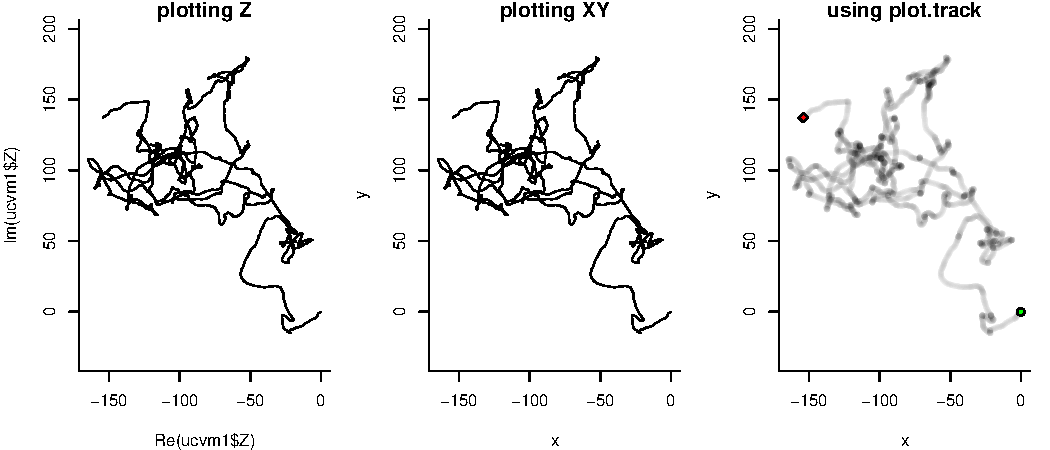
\includegraphics[width=\maxwidth]{figure/FirstPlot-1} 

\end{knitrout}
\noindent The {\tt plot\_track} function is a simple convenience function for plotting tracks.  According to theory, the mean speed of this track should just be $\nu$ = 2:

\begin{knitrout}
\definecolor{shadecolor}{rgb}{0.969, 0.969, 0.969}\color{fgcolor}\begin{kframe}
\begin{alltt}
\hlkwd{mean}\hlstd{(}\hlkwd{Mod}\hlstd{(ucvm1}\hlopt{$}\hlstd{V))}
\end{alltt}
\begin{verbatim}
## [1] 2.031516
\end{verbatim}
\end{kframe}
\end{knitrout}

\noindent and the root mean square speed should be $2 \nu / \sqrt{\pi}$ = 2.2567583:

\begin{knitrout}
\definecolor{shadecolor}{rgb}{0.969, 0.969, 0.969}\color{fgcolor}\begin{kframe}
\begin{alltt}
\hlkwd{sqrt}\hlstd{(}\hlkwd{mean}\hlstd{(}\hlkwd{Mod}\hlstd{(ucvm1}\hlopt{$}\hlstd{V)}\hlopt{^}\hlnum{2}\hlstd{))}
\end{alltt}
\begin{verbatim}
## [1] 2.288807
\end{verbatim}
\end{kframe}
\end{knitrout}

\subsubsection{Exact method}

The \emph{exact} method is more flexible, as it samples the position and velocity process simultaneously from the complete mean and variance-covariance structure of the integreated OU process.  The main advantage is that the process can be simulated for irregular (and totally arbitrary) times of observation:

\begin{knitrout}
\definecolor{shadecolor}{rgb}{0.969, 0.969, 0.969}\color{fgcolor}\begin{kframe}
\begin{alltt}
\hlstd{T} \hlkwb{<-} \hlkwd{cumsum}\hlstd{(}\hlkwd{rexp}\hlstd{(}\hlnum{100}\hlstd{))}
\hlstd{ucvm2} \hlkwb{<-} \hlkwd{simulateUCVM.exact}\hlstd{(}\hlkwc{T} \hlstd{= T,} \hlkwc{nu} \hlstd{=} \hlnum{2}\hlstd{,} \hlkwc{tau} \hlstd{=} \hlnum{2}\hlstd{)}
\hlkwd{with}\hlstd{(ucvm2,} \hlkwd{scan_track}\hlstd{(}\hlkwc{time} \hlstd{= T,} \hlkwc{z} \hlstd{= Z))}
\end{alltt}
\end{kframe}
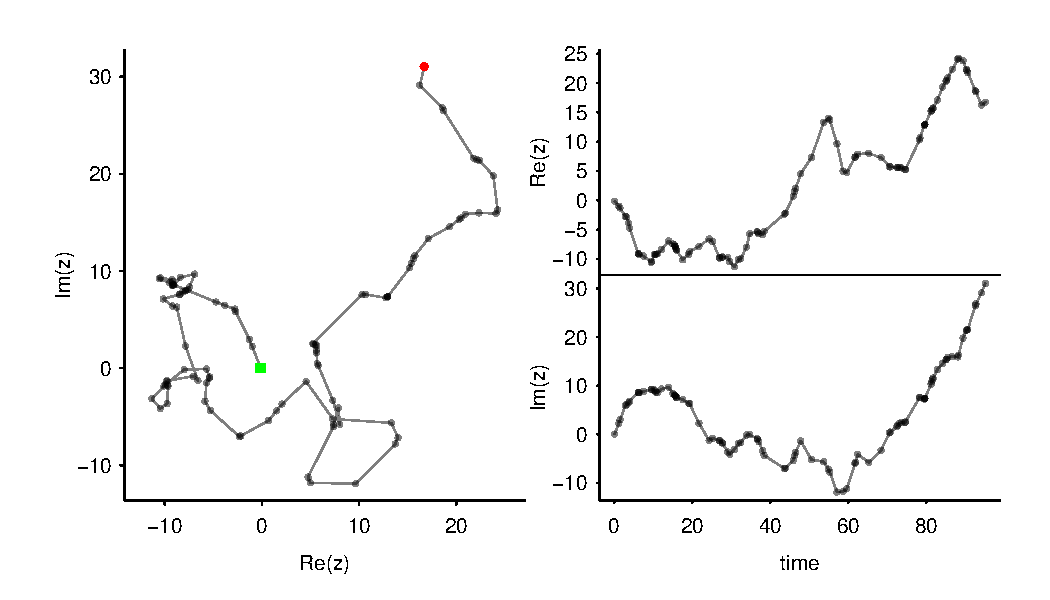
\includegraphics[width=\maxwidth]{figure/ucvm_exact-1} 

\end{knitrout}
\noindent  The \texttt{scan\_track} function is another function that is convenient for seeing a process in time (right plots).  Note the irregularity of the sampling. 
\begin{knitrout}
\definecolor{shadecolor}{rgb}{0.969, 0.969, 0.969}\color{fgcolor}\begin{kframe}
\begin{alltt}
\hlkwd{summary}\hlstd{(}\hlkwd{diff}\hlstd{(ucvm2}\hlopt{$}\hlstd{T))}
\end{alltt}
\begin{verbatim}
##     Min.  1st Qu.   Median     Mean  3rd Qu.     Max. 
## 0.001575 0.224599 0.594203 0.889439 1.305699 5.066716
\end{verbatim}
\end{kframe}
\end{knitrout}

\noindent and that the velocity vector has the correct statistical properties (mean and 95\% C.I.):
\begin{knitrout}
\definecolor{shadecolor}{rgb}{0.969, 0.969, 0.969}\color{fgcolor}\begin{kframe}
\begin{alltt}
\hlkwd{mean}\hlstd{(}\hlkwd{Mod}\hlstd{(ucvm2}\hlopt{$}\hlstd{V))}
\end{alltt}
\begin{verbatim}
## [1] 2.069103
\end{verbatim}
\begin{alltt}
\hlkwd{with}\hlstd{(ucvm2,} \hlkwd{mean}\hlstd{(}\hlkwd{Mod}\hlstd{(V))} \hlopt{+} \hlkwd{c}\hlstd{(}\hlopt{-}\hlnum{2}\hlstd{,}\hlnum{2}\hlstd{)}\hlopt{*}\hlkwd{sd}\hlstd{(}\hlkwd{Mod}\hlstd{(V))} \hlopt{/} \hlkwd{sqrt}\hlstd{(}\hlkwd{length}\hlstd{(V)))}
\end{alltt}
\begin{verbatim}
## [1] 1.869962 2.268244
\end{verbatim}
\end{kframe}
\end{knitrout}


\subsection{Rotational-Advective CVM}

The (R/A)CVM models are parameterized in terms of $\tau$, the random rms speed $\eta$, and then some combination of the advection vector $\bmu$ and/or angular speed $\omega$. 

\begin{knitrout}
\definecolor{shadecolor}{rgb}{0.969, 0.969, 0.969}\color{fgcolor}\begin{kframe}
\begin{alltt}
\hlstd{rcvm} \hlkwb{<-} \hlkwd{simulateRACVM}\hlstd{(}\hlkwc{tau} \hlstd{=} \hlnum{6}\hlstd{,} \hlkwc{eta} \hlstd{=} \hlnum{2}\hlstd{,} \hlkwc{omega} \hlstd{=} \hlnum{1}\hlstd{,} \hlkwc{mu} \hlstd{=} \hlnum{0}\hlstd{,} \hlkwc{Tmax} \hlstd{=} \hlnum{1000}\hlstd{,} \hlkwc{dt} \hlstd{=} \hlnum{.1}\hlstd{)}
\hlstd{acvm} \hlkwb{<-} \hlkwd{simulateRACVM}\hlstd{(}\hlkwc{tau} \hlstd{=} \hlnum{6}\hlstd{,} \hlkwc{eta} \hlstd{=} \hlnum{2}\hlstd{,} \hlkwc{omega} \hlstd{=} \hlnum{0}\hlstd{,} \hlkwc{mu} \hlstd{=} \hlnum{2}\hlstd{,} \hlkwc{Tmax} \hlstd{=} \hlnum{1000}\hlstd{,} \hlkwc{dt} \hlstd{=} \hlnum{.1}\hlstd{)}
\hlstd{racvm} \hlkwb{<-} \hlkwd{simulateRACVM}\hlstd{(}\hlkwc{tau} \hlstd{=} \hlnum{6}\hlstd{,} \hlkwc{eta} \hlstd{=} \hlnum{2}\hlstd{,} \hlkwc{omega} \hlstd{=} \hlnum{1}\hlstd{,} \hlkwc{mu} \hlstd{=} \hlnum{1}\hlstd{,} \hlkwc{Tmax} \hlstd{=} \hlnum{1000}\hlstd{,} \hlkwc{dt} \hlstd{=} \hlnum{.1}\hlstd{)}
\end{alltt}
\end{kframe}
\end{knitrout}

\begin{knitrout}
\definecolor{shadecolor}{rgb}{0.969, 0.969, 0.969}\color{fgcolor}\begin{kframe}
\begin{alltt}
\hlkwd{plot_track}\hlstd{(rcvm}\hlopt{$}\hlstd{Z[rcvm}\hlopt{$}\hlstd{T} \hlopt{<} \hlnum{100}\hlstd{],}  \hlkwc{main} \hlstd{=} \hlstr{"RCVM"}\hlstd{)}
\hlkwd{plot_track}\hlstd{(acvm}\hlopt{$}\hlstd{Z[acvm}\hlopt{$}\hlstd{T} \hlopt{<} \hlnum{100}\hlstd{],} \hlkwc{main} \hlstd{=} \hlstr{"ACVM"}\hlstd{)}
\hlkwd{plot_track}\hlstd{(racvm}\hlopt{$}\hlstd{Z[racvm}\hlopt{$}\hlstd{T} \hlopt{<} \hlnum{100}\hlstd{],} \hlkwc{main} \hlstd{=} \hlstr{"RACVM"}\hlstd{)}
\end{alltt}
\end{kframe}
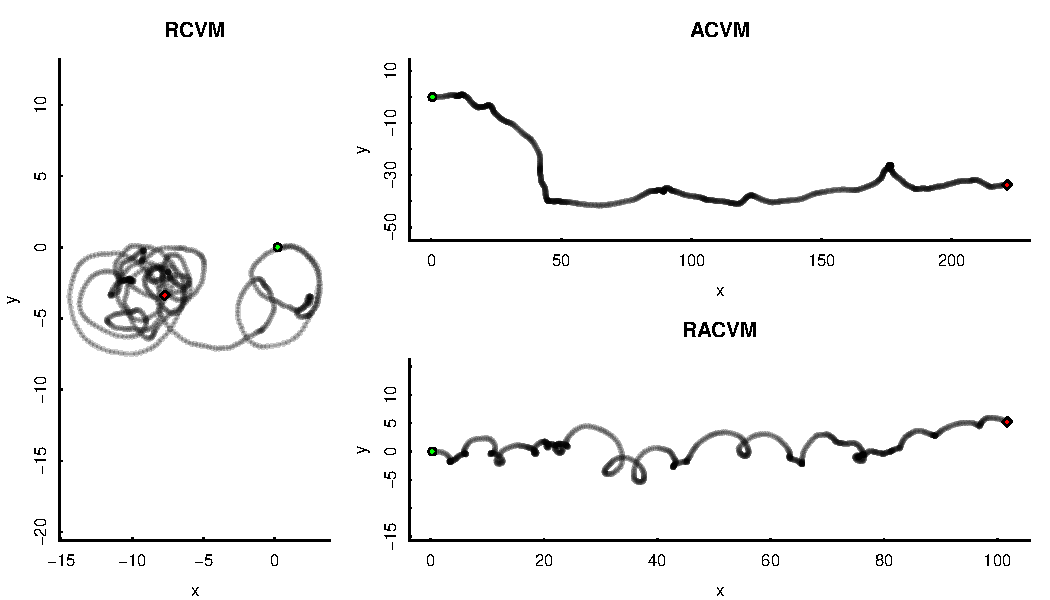
\includegraphics[width=\maxwidth]{figure/plotRACVM-1} 

\end{knitrout}

\noindent Note that we only plot these curves within the first 100 time units.  For the moment, the RACVM models can only be simulated ``directly'', i.e.~via direct forward simulations rather than sampling from the complete autocorrelated process. 

\section{Empirical velocity auto-correlation function}

The velocity autocovariance function (VAF) is a very useful way to visualize the autocorrelation structure of the movement models. It is defined as the expectation of a dot product of the velocity vector with itself as a function of lags:
\begin{eqnarray}\label{eq.VAFdefined}
			C_v(\Delta t) = \text{E}\left[ {\bf v}(t_0+\Delta t) \cdot {\bf v}(t_0) \right], \nonumber \\ 
\end{eqnarray}S
\noindent At lag 0, the value is mean squared speed of the process, and at long lags it is the square of the mean drift of the process.  For CVM models, $C_v(0) = \eta^2 + \mu^2$, $\lim_{\Delta t \to \infty} C_v(\Delta t) = \mu^2$, and the function decays exponentially at rate $\tau$ with an oscillatory component with angular velocity $\omega$. The main functions for computing the empirical VAF is the \texttt{getEVAF} function:

\begin{knitrout}
\definecolor{shadecolor}{rgb}{0.969, 0.969, 0.969}\color{fgcolor}\begin{kframe}
\begin{alltt}
\hlstd{ucvm.vaf} \hlkwb{<-} \hlkwd{with}\hlstd{(ucvm1,} \hlkwd{getEVAF}\hlstd{(}\hlkwc{Z} \hlstd{= Z,} \hlkwc{T} \hlstd{= T,} \hlkwc{lagmax} \hlstd{=} \hlnum{30}\hlstd{))}
\hlstd{acvm.vaf} \hlkwb{<-} \hlkwd{with}\hlstd{(acvm,} \hlkwd{getEVAF}\hlstd{(}\hlkwc{Z} \hlstd{= Z,} \hlkwc{T} \hlstd{= T,} \hlkwc{lagmax} \hlstd{=} \hlnum{30}\hlstd{))}
\hlstd{rcvm.vaf} \hlkwb{<-} \hlkwd{with}\hlstd{(rcvm,} \hlkwd{getEVAF}\hlstd{(}\hlkwc{Z} \hlstd{= Z,} \hlkwc{T} \hlstd{= T,} \hlkwc{lagmax} \hlstd{=} \hlnum{30}\hlstd{))}
\hlstd{racvm.vaf} \hlkwb{<-} \hlkwd{with}\hlstd{(racvm,} \hlkwd{getEVAF}\hlstd{(}\hlkwc{Z} \hlstd{= Z,} \hlkwc{T} \hlstd{= T,} \hlkwc{lagmax} \hlstd{=} \hlnum{30}\hlstd{))}
\end{alltt}
\end{kframe}
\end{knitrout}

\noindent This function produces a two column data frame with the lag and the respective computed evaf:
\begin{knitrout}
\definecolor{shadecolor}{rgb}{0.969, 0.969, 0.969}\color{fgcolor}\begin{kframe}
\begin{alltt}
\hlkwd{head}\hlstd{(ucvm.vaf)}
\end{alltt}
\begin{verbatim}
##   lag      vaf
## 1 0.0 5.238760
## 2 0.1 5.136165
## 3 0.2 5.034438
## 4 0.3 4.933219
## 5 0.4 4.833052
## 6 0.5 4.734453
\end{verbatim}
\end{kframe}
\end{knitrout}

\noindent A plot of the four curves and their respective empirical autocovariance functions:

\begin{knitrout}
\definecolor{shadecolor}{rgb}{0.969, 0.969, 0.969}\color{fgcolor}\begin{kframe}
\begin{alltt}
\hlkwd{plot_track}\hlstd{(ucvm1}\hlopt{$}\hlstd{Z[}\hlnum{1}\hlopt{:}\hlnum{1e3}\hlstd{],} \hlkwc{main} \hlstd{=} \hlstr{"UCVM"}\hlstd{);} \hlkwd{plot}\hlstd{(ucvm.vaf,} \hlkwc{type}\hlstd{=}\hlstr{"l"}\hlstd{,} \hlkwc{lwd}\hlstd{=}\hlnum{1.5}\hlstd{)}
\hlkwd{plot_track}\hlstd{(acvm}\hlopt{$}\hlstd{Z[}\hlnum{1}\hlopt{:}\hlnum{1e3}\hlstd{],} \hlkwc{main} \hlstd{=} \hlstr{"ACVM"}\hlstd{);} \hlkwd{plot}\hlstd{(acvm.vaf,} \hlkwc{type}\hlstd{=}\hlstr{"l"}\hlstd{,} \hlkwc{lwd}\hlstd{=}\hlnum{1.5}\hlstd{)}
\hlkwd{plot_track}\hlstd{(rcvm}\hlopt{$}\hlstd{Z[}\hlnum{1}\hlopt{:}\hlnum{1e3}\hlstd{],} \hlkwc{main} \hlstd{=} \hlstr{"RCVM"}\hlstd{);} \hlkwd{plot}\hlstd{(rcvm.vaf,} \hlkwc{type}\hlstd{=}\hlstr{"l"}\hlstd{,} \hlkwc{lwd}\hlstd{=}\hlnum{1.5}\hlstd{)}
\hlkwd{plot_track}\hlstd{(racvm}\hlopt{$}\hlstd{Z[}\hlnum{1}\hlopt{:}\hlnum{1e3}\hlstd{],} \hlkwc{main} \hlstd{=} \hlstr{"RACVM"}\hlstd{);} \hlkwd{plot}\hlstd{(racvm.vaf,} \hlkwc{type}\hlstd{=}\hlstr{"l"}\hlstd{,} \hlkwc{lwd}\hlstd{=}\hlnum{1.5}\hlstd{)}
\end{alltt}
\end{kframe}
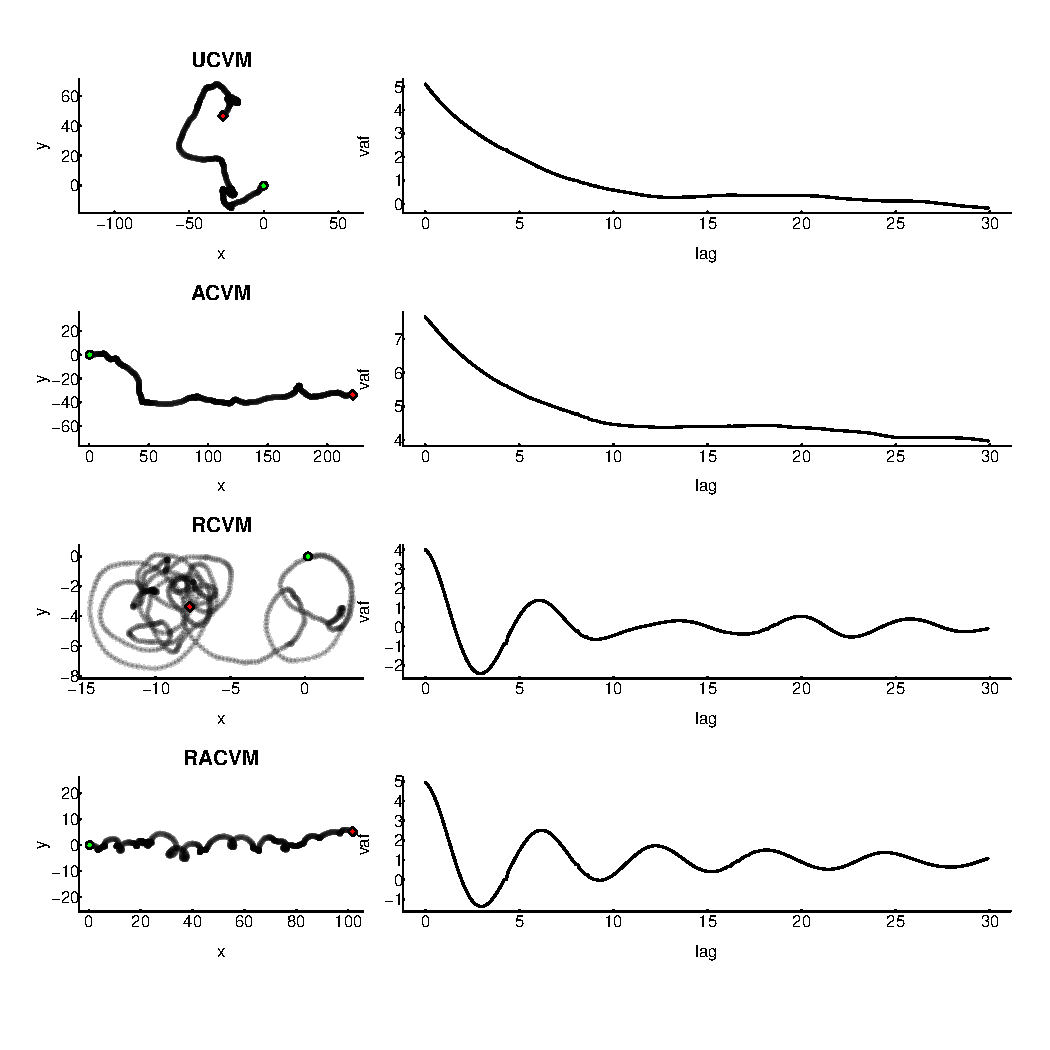
\includegraphics[width=\maxwidth]{figure/EVAFplots-1} 

\end{knitrout}

\noindent The velocity autocovariance functions is a very useful visual summary of a movement track because it refeals . Furthermore These curves can be used to estimate the parameters of these processes. 

\section{Estimation of CVM models}

The main estimation functions are \texttt{estimateUCVM} and \texttt{estimateRACVM}.  The respective help files have abundant examples of implementation. 

\subsection{UCVM}

Following the structure of the Gurarie at al.~(\emph{in review}), manuscript, the UCVM, which focusses on estimates of time scale $\tau$ and speed $\nu$, can be estimated using one of five different methods.

\subsubsection{VAF fitting}

This method relies on fitting the \emph{empirical} velocity autocorrelation function (above) to the \emph{theoretical} velocity autocorrelation function:
$$C_v(\Delta t) = {4 \over \pi} \nu^2 \exp(\Delta t / \tau)$$

\begin{knitrout}
\definecolor{shadecolor}{rgb}{0.969, 0.969, 0.969}\color{fgcolor}\begin{kframe}
\begin{alltt}
\hlkwd{estimateUCVM}\hlstd{(}\hlkwc{Z} \hlstd{= ucvm1}\hlopt{$}\hlstd{Z,} \hlkwc{T} \hlstd{= ucvm1}\hlopt{$}\hlstd{T,} \hlkwc{method} \hlstd{=} \hlstr{"vaf"}\hlstd{,} \hlkwc{diagnose} \hlstd{=} \hlnum{TRUE}\hlstd{,} \hlkwc{CI}\hlstd{=}\hlnum{TRUE}\hlstd{)}
\end{alltt}
\end{kframe}
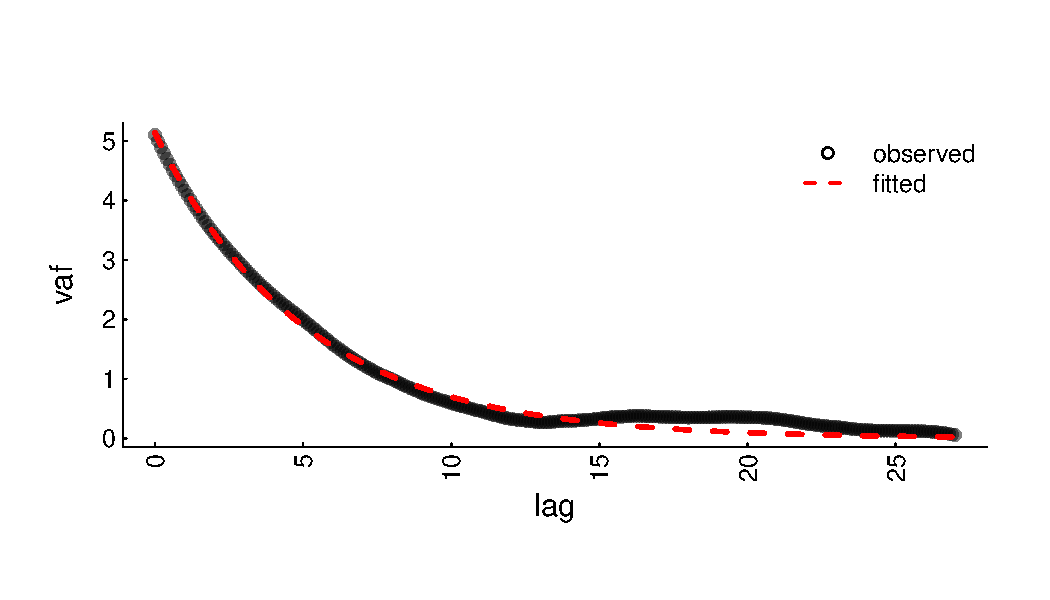
\includegraphics[width=\maxwidth]{figure/VAF1-1} 
\begin{kframe}\begin{verbatim}
##     Estimate  C.I.low C.I.high
## tau 4.858959 4.791005 4.928869
## nu  2.031519 1.802198 2.260839
\end{verbatim}
\end{kframe}
\end{knitrout}
\noindent The diagnostic plot (only plotted with \texttt{diagnose=TRUE}) illustrates the quality of the fit.  The estimates should be fairly good, when compared to the true parameters: 
\begin{knitrout}
\definecolor{shadecolor}{rgb}{0.969, 0.969, 0.969}\color{fgcolor}\begin{kframe}
\begin{alltt}
\hlstd{ucvm1}\hlopt{$}\hlstd{parameters[}\hlnum{1}\hlopt{:}\hlnum{2}\hlstd{]}
\end{alltt}
\begin{verbatim}
## $tau
## [1] 5
## 
## $nu
## [1] 2
\end{verbatim}
\end{kframe}
\end{knitrout}
\noindent A lower-resolution track will have wider confidence intervals:
\begin{knitrout}
\definecolor{shadecolor}{rgb}{0.969, 0.969, 0.969}\color{fgcolor}\begin{kframe}
\begin{alltt}
\hlstd{ucvm.lores} \hlkwb{<-} \hlkwd{simulateUCVM}\hlstd{(}\hlkwc{nu}\hlstd{=}\hlnum{10}\hlstd{,} \hlkwc{tau} \hlstd{=} \hlnum{4}\hlstd{,} \hlkwc{dt} \hlstd{=} \hlnum{1}\hlstd{,} \hlkwc{T.max} \hlstd{=} \hlnum{1000}\hlstd{,} \hlkwc{method} \hlstd{=} \hlstr{"exact"}\hlstd{)}
\hlkwd{with}\hlstd{(ucvm.lores,} \hlkwd{estimateUCVM}\hlstd{(}\hlkwc{Z} \hlstd{= Z,} \hlkwc{T} \hlstd{= T,} \hlkwc{CI}\hlstd{=}\hlnum{TRUE}\hlstd{,} \hlkwc{method}\hlstd{=}\hlstr{"vaf"}\hlstd{))}
\end{alltt}
\begin{verbatim}
##     Estimate  C.I.low C.I.high
## tau 4.330770 3.761759 5.102600
## nu  9.352172 8.894749 9.809595
\end{verbatim}
\end{kframe}
\end{knitrout}
\noindent The speed estimate might be improved by using a spline correction
\begin{knitrout}
\definecolor{shadecolor}{rgb}{0.969, 0.969, 0.969}\color{fgcolor}\begin{kframe}
\begin{alltt}
\hlkwd{with}\hlstd{(ucvm.lores,} \hlkwd{estimateUCVM}\hlstd{(}\hlkwc{Z} \hlstd{= Z,} \hlkwc{T} \hlstd{= T,} \hlkwc{CI}\hlstd{=}\hlnum{TRUE}\hlstd{,} \hlkwc{method}\hlstd{=}\hlstr{"vaf"}\hlstd{,} \hlkwc{spline} \hlstd{=} \hlnum{TRUE}\hlstd{))}
\end{alltt}
\begin{verbatim}
##     Estimate  C.I.low C.I.high
## tau 3.980474 3.548952 4.531460
## nu  9.574312 9.194147 9.954476
\end{verbatim}
\end{kframe}
\end{knitrout}

\noindent \emph{NB: This method works only for regularly sampled data, and the confidence intervals tend to be unreliable.}

\subsubsection{CRW matching}

The Correlated Random Walk (CRW) matching method computes the CRW parameters (shape and scale of length steps and wrapped Cauchy clustering coefficient) and converts those to time-scales and speed estimates.  Confidence intervals are obtained by Monte Carlo draws from the confidence intervals around likelihood estimates of the CRW parameters.  

\begin{knitrout}
\definecolor{shadecolor}{rgb}{0.969, 0.969, 0.969}\color{fgcolor}\begin{kframe}
\begin{alltt}
  \hlstd{tau} \hlkwb{<-} \hlnum{2}\hlstd{; nu} \hlkwb{<-} \hlnum{8}
  \hlstd{ucvm3} \hlkwb{<-} \hlkwd{simulateUCVM}\hlstd{(}\hlkwc{T}\hlstd{=}\hlnum{1}\hlopt{:}\hlnum{1000}\hlstd{,} \hlkwc{nu} \hlstd{= nu,} \hlkwc{tau} \hlstd{= tau,} \hlkwc{method} \hlstd{=} \hlstr{"exact"}\hlstd{)}
  \hlkwd{plot}\hlstd{(ucvm3}\hlopt{$}\hlstd{Z,} \hlkwc{asp}\hlstd{=}\hlnum{1}\hlstd{,} \hlkwc{type}\hlstd{=}\hlstr{"o"}\hlstd{,} \hlkwc{cex}\hlstd{=}\hlnum{0.5}\hlstd{,} \hlkwc{pch}\hlstd{=}\hlnum{19}\hlstd{)}
\end{alltt}
\end{kframe}

{\centering 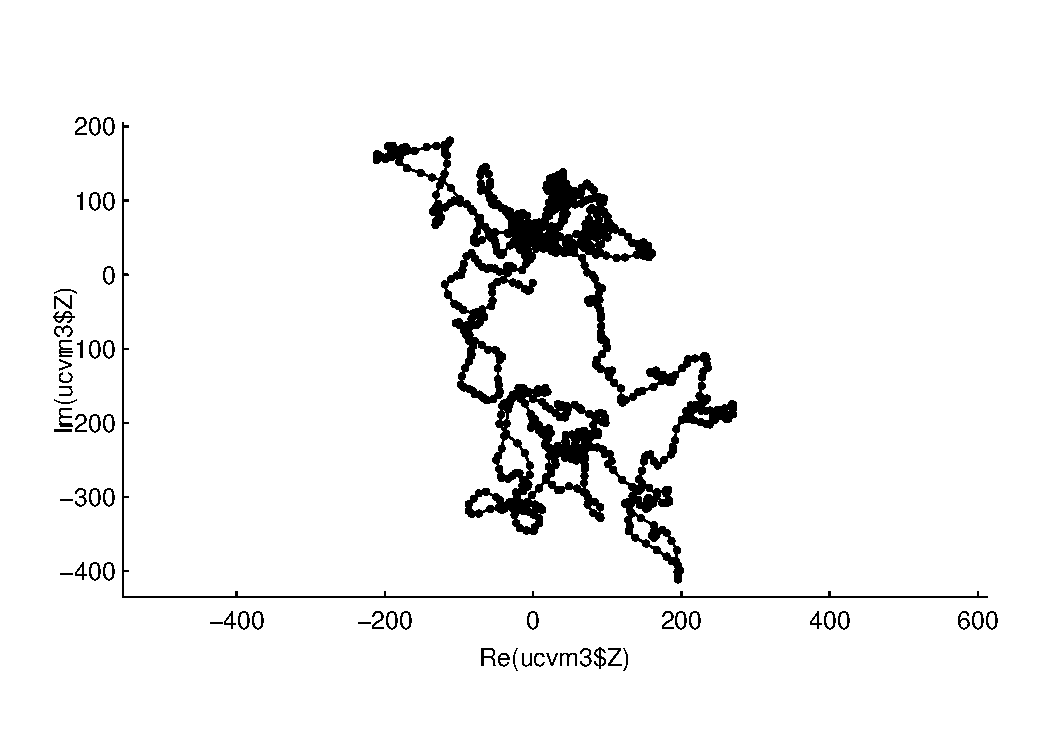
\includegraphics[width=4in]{figure/CRW-1} 

}


\begin{kframe}\begin{alltt}
  \hlkwd{estimateUCVM}\hlstd{(}\hlkwc{Z} \hlstd{= ucvm3}\hlopt{$}\hlstd{Z,} \hlkwc{T} \hlstd{= ucvm3}\hlopt{$}\hlstd{T,} \hlkwc{CI}\hlstd{=}\hlnum{TRUE}\hlstd{,} \hlkwc{method}\hlstd{=}\hlstr{"crw"}\hlstd{,} \hlkwc{diagnose}\hlstd{=}\hlnum{TRUE}\hlstd{)}
\end{alltt}
\end{kframe}

{\centering 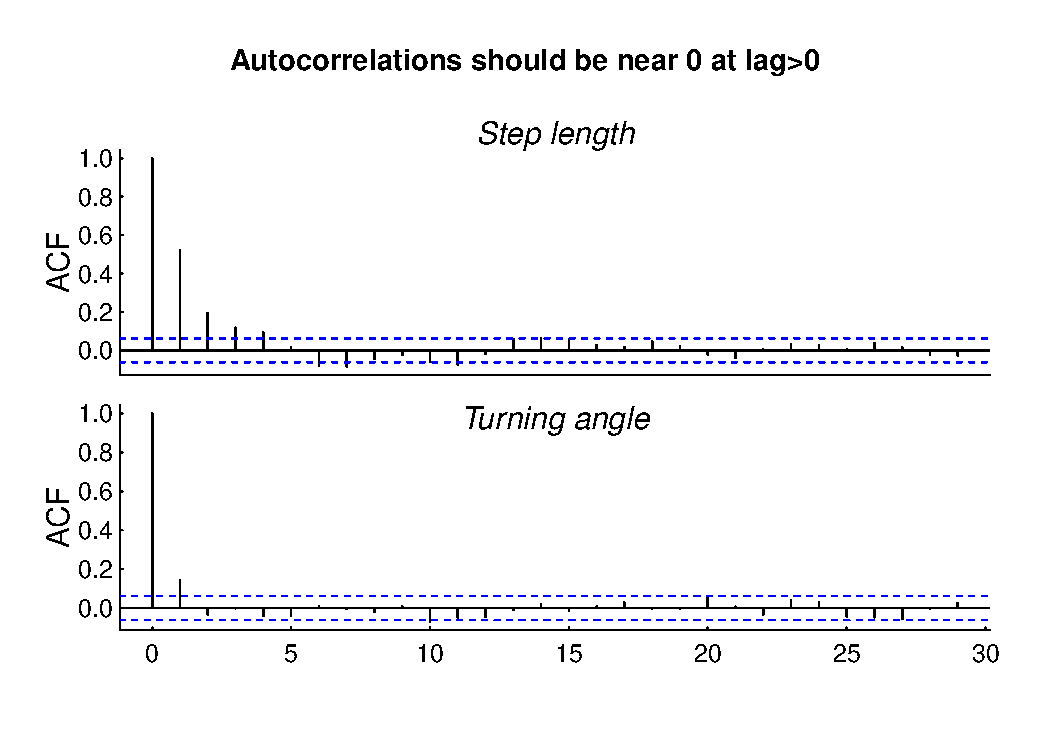
\includegraphics[width=4in]{figure/CRW-2} 

}


\begin{kframe}\begin{verbatim}
##     Estimate  C.I.low C.I.high
## tau 1.992912 1.779502 2.293856
## nu  6.661996 6.081514 7.174524
\end{verbatim}
\end{kframe}
\end{knitrout}
\noindent The diagnosis plots (crudely) illustrates the standard autocorrelation function for the step lengths and turning angles.  Under the normal assumptions of the CRW, these should both be around 0 at lags greater than 0.  The more autocorrelated either of these time series is, the more biased the estimates are likely to be. 

\noindent\emph{NB: This method is illustrative, generally biased, and not recommended except for data that are relatively coarsely sampled.  It is, however, very fast to compute.}

\subsubsection{Velocity likelihood}

The velocity likelihood method is based on using the known distributional properties of the integrated OU obtain a "one-step" likelihood of each velocity based on the previous velocity.  This method is robust to irregularly sampled data and is fairly fast.  We will estimate the original track 

\begin{knitrout}
\definecolor{shadecolor}{rgb}{0.969, 0.969, 0.969}\color{fgcolor}\begin{kframe}
\begin{alltt}
\hlkwd{estimateUCVM}\hlstd{(}\hlkwc{Z} \hlstd{= ucvm1}\hlopt{$}\hlstd{Z,} \hlkwc{T} \hlstd{= ucvm1}\hlopt{$}\hlstd{T,} \hlkwc{method} \hlstd{=} \hlstr{"vLike"}\hlstd{,} \hlkwc{CI}\hlstd{=}\hlnum{TRUE}\hlstd{)}
\end{alltt}
\begin{verbatim}
##     Estimate  C.I.low C.I.high
## tau 5.035226 4.375848 5.793963
## nu  2.026834 1.885991 2.167676
\end{verbatim}
\end{kframe}
\end{knitrout}

\noindent  This method gives very reliable confidence intervals, but may underestimate velocities. We can also run it on the irregularly sampled track from above:
\begin{knitrout}
\definecolor{shadecolor}{rgb}{0.969, 0.969, 0.969}\color{fgcolor}\begin{kframe}
\begin{alltt}
\hlkwd{estimateUCVM}\hlstd{(}\hlkwc{Z} \hlstd{= ucvm2}\hlopt{$}\hlstd{Z,} \hlkwc{T} \hlstd{= ucvm2}\hlopt{$}\hlstd{T,} \hlkwc{method} \hlstd{=} \hlstr{"vLike"}\hlstd{,} \hlkwc{CI}\hlstd{=}\hlnum{TRUE}\hlstd{)}
\end{alltt}
\begin{verbatim}
##     Estimate  C.I.low C.I.high
## tau 2.826492 1.863552 4.287003
## nu  1.802529 1.475147 2.129912
\end{verbatim}
\end{kframe}
\end{knitrout}
\noindent The confidence intervals are more wide this time (due to a much smaller data set: 100 versus 10001 data points), but the estimates should be fairly accurate. 

\subsubsection{Position likelihood}

The position likelihood (\texttt{zLike}) takes the complete correlation structure between the velocities and the positions to estimate the parameters.  It is prohibitively slow on a data set the size of \texttt{ucvm1}, but quite fast on the second (irregular, short) sampling: 

\begin{knitrout}
\definecolor{shadecolor}{rgb}{0.969, 0.969, 0.969}\color{fgcolor}\begin{kframe}
\begin{alltt}
\hlkwd{estimateUCVM}\hlstd{(}\hlkwc{Z} \hlstd{= ucvm2}\hlopt{$}\hlstd{Z,} \hlkwc{T} \hlstd{= ucvm2}\hlopt{$}\hlstd{T,} \hlkwc{method} \hlstd{=} \hlstr{"zLike"}\hlstd{,} \hlkwc{CI}\hlstd{=}\hlnum{TRUE}\hlstd{)}
\end{alltt}
\begin{verbatim}
##     Estimate   C.I.low C.I.high
## tau 1.799556  1.268449 2.553041
## nu  1.953387  1.570523 2.336250
## v0x 1.051625 -1.244793 3.348044
## v0y 3.160491  0.864072 5.456909
\end{verbatim}
\end{kframe}
\end{knitrout}
\noindent Note, improvements in the parameter estimates and confidence intervals, and the inclusion of estimates for the initial speed (usually a parameter of less interest). 

\subsubsection{Position likelihood: Kalman filter}

We (OO and EG) had independently worked out many of the details of the estimation of full position likelihood before we discovered that the same likelihood was estimated in a much more efficient way by Johnson et al. (2008), and encoded in an excellent package called ``crawl'' (\emph{Correlated RAndom Walk Library}).  We have incorporated a wrapper for this package in \texttt{smoove} for the estimation of UCVM parameters - a fairly narrow application of the capabilities of \texttt{crawl}.  First, we run it on the irregular data set:
\begin{knitrout}
\definecolor{shadecolor}{rgb}{0.969, 0.969, 0.969}\color{fgcolor}\begin{kframe}
\begin{alltt}
\hlkwd{with}\hlstd{(ucvm2,} \hlkwd{estimateUCVM}\hlstd{(}\hlkwc{Z} \hlstd{= Z,} \hlkwc{T} \hlstd{= T,} \hlkwc{method} \hlstd{=} \hlstr{"crawl"}\hlstd{))}
\end{alltt}


{\ttfamily\noindent\itshape\color{messagecolor}{\#\# Beginning SANN initialization ...}}

{\ttfamily\noindent\itshape\color{messagecolor}{\#\# Beginning likelihood optimization ...}}\begin{verbatim}
## 
## 
## Continuous-Time Correlated Random Walk fit
## 
## Models:
## --------
## Movement   ~ 1
## Error   
## 
## 
##                      Parameter Est. St. Err. 95% Lower 95% Upper
## ln sigma (Intercept)          1.090    0.152     0.793     1.388
## ln beta (Intercept)          -0.585    0.181     -0.94    -0.231
## 
## 
## Log Likelihood = 85.236 
## AIC = -166.472
##     Estimate        L        U
## tau 1.795195 1.259472 2.558792
## nu  1.968246 1.462124 2.649563
\end{verbatim}
\end{kframe}
\end{knitrout}
\noindent The estimates and C.I.'s for $\nu$ and $\tau$ are very similar to the full position likelihood above.   The additional output is specific to the parameterization Johnson et al.~use, the lower output (\texttt{nutau}) is consistent with the output for the other methods.  

\noindent The \texttt{crawl} method can handle a very long ($n = 10000$) dataset as well.  

\begin{knitrout}
\definecolor{shadecolor}{rgb}{0.969, 0.969, 0.969}\color{fgcolor}\begin{kframe}
\begin{alltt}
\hlkwd{with}\hlstd{(ucvm1,} \hlkwd{estimateUCVM}\hlstd{(}\hlkwc{Z} \hlstd{= Z,} \hlkwc{T} \hlstd{= T,} \hlkwc{method} \hlstd{=} \hlstr{"crawl"}\hlstd{))}
\end{alltt}


{\ttfamily\noindent\itshape\color{messagecolor}{\#\# Beginning SANN initialization ...}}

{\ttfamily\noindent\itshape\color{messagecolor}{\#\# Beginning likelihood optimization ...}}\begin{verbatim}
## 
## 
## Continuous-Time Correlated Random Walk fit
## 
## Models:
## --------
## Movement   ~ 1
## Error   
## 
## 
##                      Parameter Est. St. Err. 95% Lower 95% Upper
## ln sigma (Intercept)          1.368    0.054     1.262     1.474
## ln beta (Intercept)          -1.069    0.055    -1.177    -0.962
## 
## 
## Log Likelihood = 58195.74 
## AIC = -116387.481
##     Estimate        L        U
## tau 2.913263 2.616068 3.244220
## nu  2.038729 1.833277 2.267206
\end{verbatim}
\end{kframe}
\end{knitrout}

\noindent with correspondingly smaller confidence intervals. There are many additional options that can be passed to the \texttt{crawl} solver, detailed in the help file for \texttt{crwMLE}.  

\subsection{RACVM}

Estimating the RACVM processes is different mainly in that there are now four different models to compare (with and without each of rotation and advection), and a model selection method is intrinsically built in.  For the time being, the method implemented for fitting these models is the \emph{velocity likelihood}.  

\noindent In the examples below, we estimate the parameters from each of the RACVM simulations and them from a portion of actual kestrel flight data:

\begin{knitrout}
\definecolor{shadecolor}{rgb}{0.969, 0.969, 0.969}\color{fgcolor}\begin{kframe}
\begin{alltt}
\hlstd{ucvm} \hlkwb{<-} \hlkwd{simulateRACVM}\hlstd{(}\hlkwc{tau} \hlstd{=} \hlnum{5}\hlstd{,} \hlkwc{eta} \hlstd{=} \hlnum{2}\hlstd{,} \hlkwc{omega} \hlstd{=} \hlnum{0}\hlstd{,} \hlkwc{mu} \hlstd{=} \hlnum{0}\hlstd{,} \hlkwc{Tmax} \hlstd{=} \hlnum{100}\hlstd{,} \hlkwc{dt} \hlstd{=} \hlnum{.1}\hlstd{)}
\hlstd{acvm} \hlkwb{<-} \hlkwd{simulateRACVM}\hlstd{(}\hlkwc{tau} \hlstd{=} \hlnum{5}\hlstd{,} \hlkwc{eta} \hlstd{=} \hlnum{2}\hlstd{,} \hlkwc{omega} \hlstd{=} \hlnum{0}\hlstd{,} \hlkwc{mu} \hlstd{=} \hlnum{2}\hlstd{,} \hlkwc{Tmax} \hlstd{=} \hlnum{100}\hlstd{,} \hlkwc{dt} \hlstd{=} \hlnum{.1}\hlstd{)}
\hlstd{rcvm} \hlkwb{<-} \hlkwd{simulateRACVM}\hlstd{(}\hlkwc{tau} \hlstd{=} \hlnum{5}\hlstd{,} \hlkwc{eta} \hlstd{=} \hlnum{2}\hlstd{,} \hlkwc{omega} \hlstd{=} \hlnum{2}\hlstd{,} \hlkwc{mu} \hlstd{=} \hlnum{0}\hlstd{,} \hlkwc{Tmax} \hlstd{=} \hlnum{100}\hlstd{,} \hlkwc{dt} \hlstd{=} \hlnum{.1}\hlstd{)}
\hlstd{racvm} \hlkwb{<-} \hlkwd{simulateRACVM}\hlstd{(}\hlkwc{tau} \hlstd{=} \hlnum{5}\hlstd{,} \hlkwc{eta} \hlstd{=} \hlnum{2}\hlstd{,} \hlkwc{omega} \hlstd{=} \hlnum{2}\hlstd{,} \hlkwc{mu} \hlstd{=} \hlnum{2}\hlstd{,} \hlkwc{Tmax} \hlstd{=} \hlnum{100}\hlstd{,} \hlkwc{dt} \hlstd{=} \hlnum{.1}\hlstd{)}
\end{alltt}
\end{kframe}
\end{knitrout}

\subsubsection{Unbiased CVM}
\begin{minipage}{0.4\linewidth}  
\begin{knitrout}
\definecolor{shadecolor}{rgb}{0.969, 0.969, 0.969}\color{fgcolor}
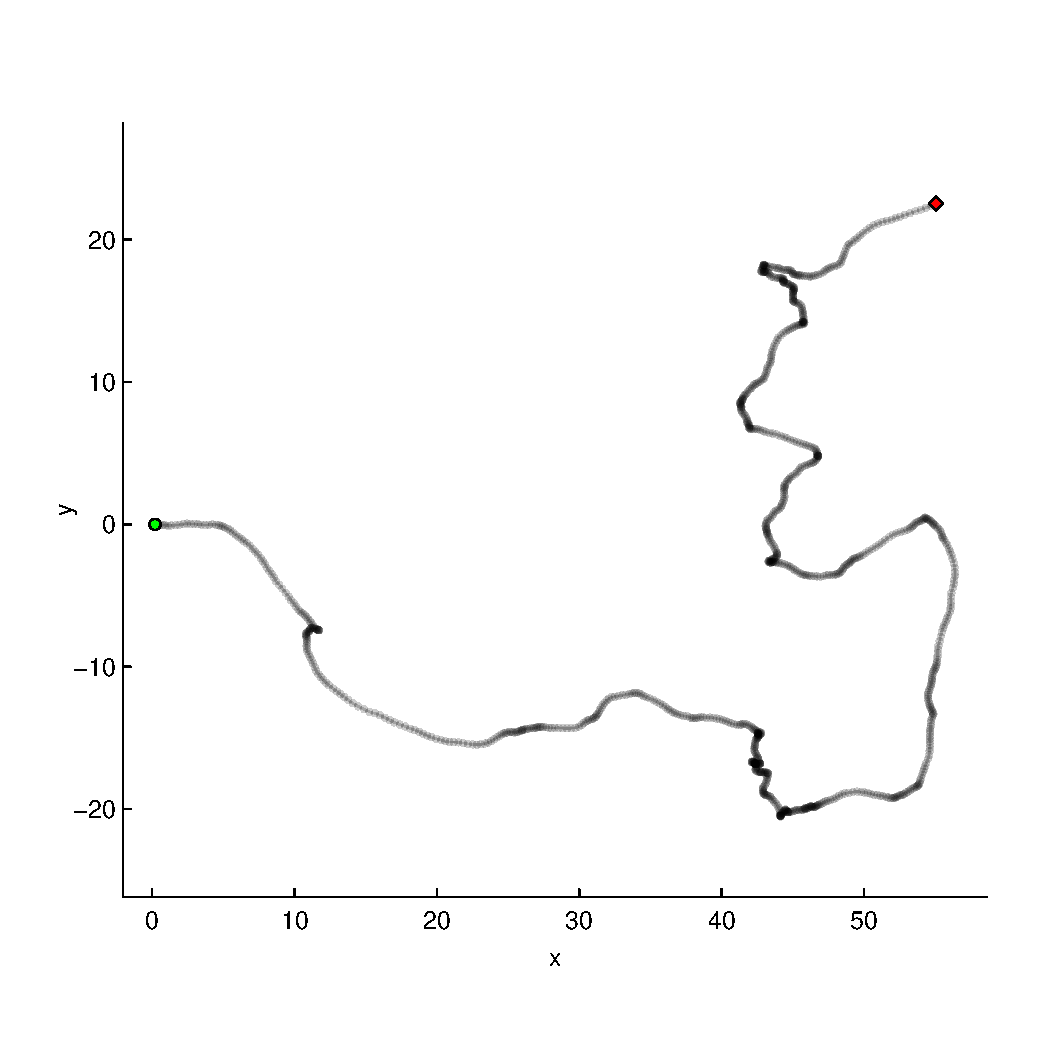
\includegraphics[width=\maxwidth]{figure/ucvm-1} 

\end{knitrout}
\end{minipage}
\begin{minipage}{0.6\linewidth}
\begin{knitrout}\small
\definecolor{shadecolor}{rgb}{0.969, 0.969, 0.969}\color{fgcolor}\begin{kframe}
\begin{alltt}
\hlkwd{with}\hlstd{(ucvm,} \hlkwd{estimateRACVM}\hlstd{(}\hlkwc{Z}\hlstd{=Z,} \hlkwc{T}\hlstd{=T,} \hlkwc{compare.models}\hlstd{=}\hlnum{TRUE}\hlstd{))}
\end{alltt}
\begin{verbatim}
## $results
##               eta       omega       mu.x       mu.y      tau      rms
## Estimate 1.706008  0.03174857  0.2129594 -1.0759083 3.506698 2.072366
## CI.low   1.383267 -0.07776853 -0.4245069 -1.7133763 2.388803 1.633966
## CI.high  2.028749  0.14126567  0.8504257 -0.4384404 5.147736 2.510766
## 
## $LL
## [1] -320.2632
## 
## $CompareTable
##         logLike k      AIC deltaAIC      BIC  deltaBIC
## UCVM  -324.7869 2 653.5738 4.711784 663.3893  0.000000
## ACVM  -320.4310 4 648.8620 0.000000 668.4930  5.103726
## RCVM  -324.5393 3 655.0786 6.216608 669.8019  6.412580
## RACVM -320.2632 5 650.5264 1.664399 675.0652 11.675880
\end{verbatim}
\end{kframe}
\end{knitrout}
\end{minipage}

\noindent The estimation function (by default) fits the most complex RACVM model.  The comparison table indicates that the most parsimonious model, according to both AIC and the more conservative BIC, is the UCVM.  Note, also, that the confidence intervals around $\omega$, $\mu_x$ and $\mu_y$ all include 0 - additional evidence that the model may not be advective or rotational.  The following code estimates the ``selected'' model.  

\begin{knitrout}
\definecolor{shadecolor}{rgb}{0.969, 0.969, 0.969}\color{fgcolor}\begin{kframe}
\begin{alltt}
\hlkwd{with}\hlstd{(ucvm,} \hlkwd{estimateRACVM}\hlstd{(}\hlkwc{Z}\hlstd{=Z,} \hlkwc{T}\hlstd{=T,} \hlkwc{model}\hlstd{=}\hlstr{"UCVM"}\hlstd{,} \hlkwc{compare.models}\hlstd{=}\hlnum{FALSE}\hlstd{))}
\end{alltt}
\begin{verbatim}
## $results
##               eta      tau      rms
## Estimate 2.030165 4.984732 2.030165
## CI.low   1.567436 3.144865 1.567436
## CI.high  2.492894 7.900992 2.492894
## 
## $LL
## [1] -324.7869
\end{verbatim}
\end{kframe}
\end{knitrout}

\noindent Every time this document is compiled, the results change somewhat.  But in most cases the model selection should return the correct model and the estimated confidence intervals should include the true values. 

\subsubsection{Advective CVM}
\begin{minipage}{0.4\linewidth}   
\begin{knitrout}
\definecolor{shadecolor}{rgb}{0.969, 0.969, 0.969}\color{fgcolor}
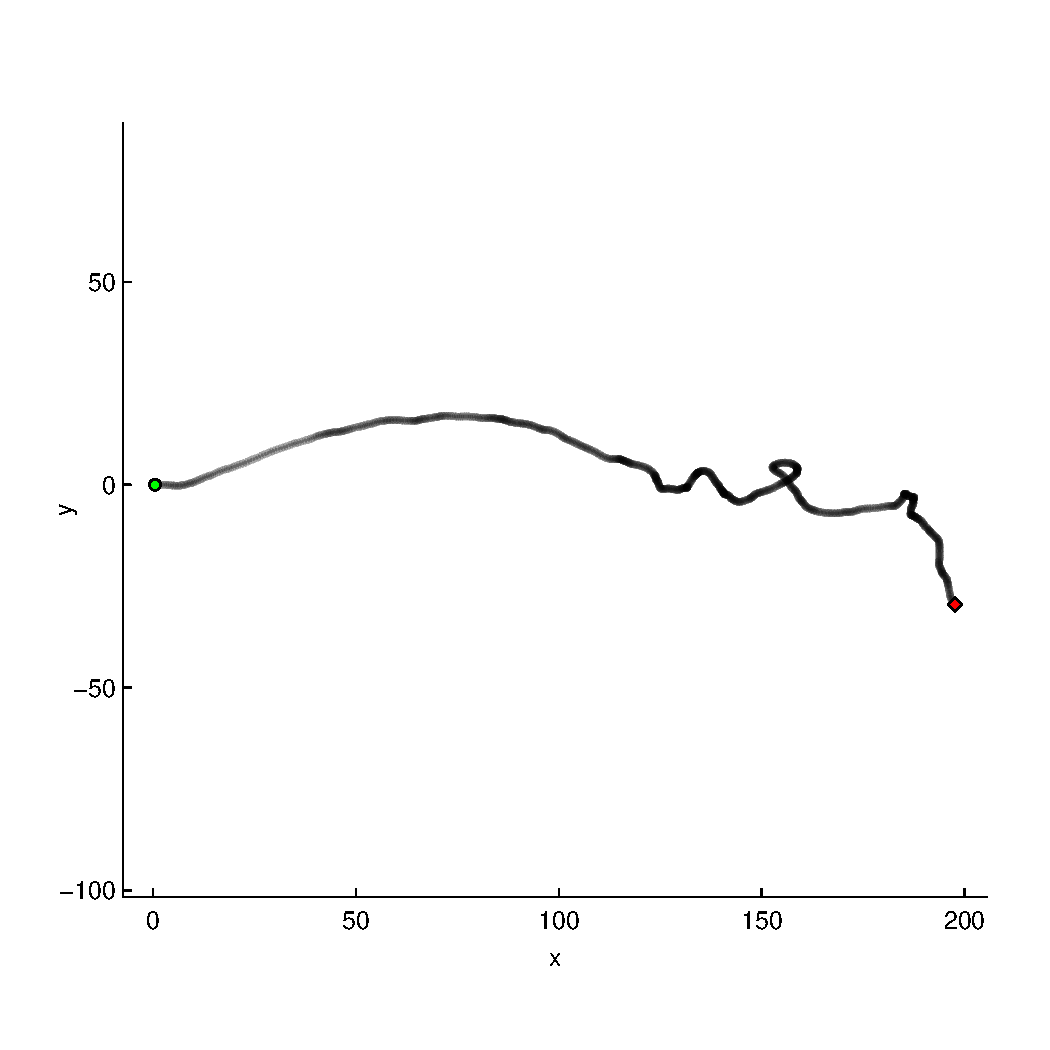
\includegraphics[width=\maxwidth]{figure/acvm-1} 

\end{knitrout}
  \end{minipage}
  \begin{minipage}{0.6\linewidth}
\begin{knitrout}\small
\definecolor{shadecolor}{rgb}{0.969, 0.969, 0.969}\color{fgcolor}\begin{kframe}
\begin{alltt}
\hlkwd{with}\hlstd{(acvm,} \hlkwd{estimateRACVM}\hlstd{(}\hlkwc{Z}\hlstd{=Z,} \hlkwc{T}\hlstd{=T,} \hlkwc{model} \hlstd{=} \hlstr{"ACVM"}\hlstd{,}
                         \hlkwc{compare.models}\hlstd{=}\hlnum{TRUE}\hlstd{))}
\end{alltt}
\begin{verbatim}
## $results
##               eta     mu.x        mu.y      tau      rms
## Estimate 1.870189 2.156809 -0.05208218 4.309585 2.896652
## CI.low   1.489074 1.377325 -0.82907917 2.853999 2.261046
## CI.high  2.251305 2.936293  0.72491482 6.507544 3.532257
## 
## $LL
## [1] -303.1154
## 
## $CompareTable
##         logLike k      AIC   deltaAIC      BIC deltaBIC
## UCVM  -309.3298 2 622.6595  9.2285851 632.4750 0.000000
## ACVM  -303.1154 4 614.2309  0.7999298 633.8619 1.386855
## RCVM  -308.8182 3 623.6364 10.2054900 638.3597 5.884660
## RACVM -301.7155 5 613.4310  0.0000000 637.9697 5.494681
\end{verbatim}
\end{kframe}
\end{knitrout}
  \end{minipage}


\subsubsection{Rotational CVM}
     \begin{minipage}{0.4\linewidth}   
\begin{knitrout}
\definecolor{shadecolor}{rgb}{0.969, 0.969, 0.969}\color{fgcolor}
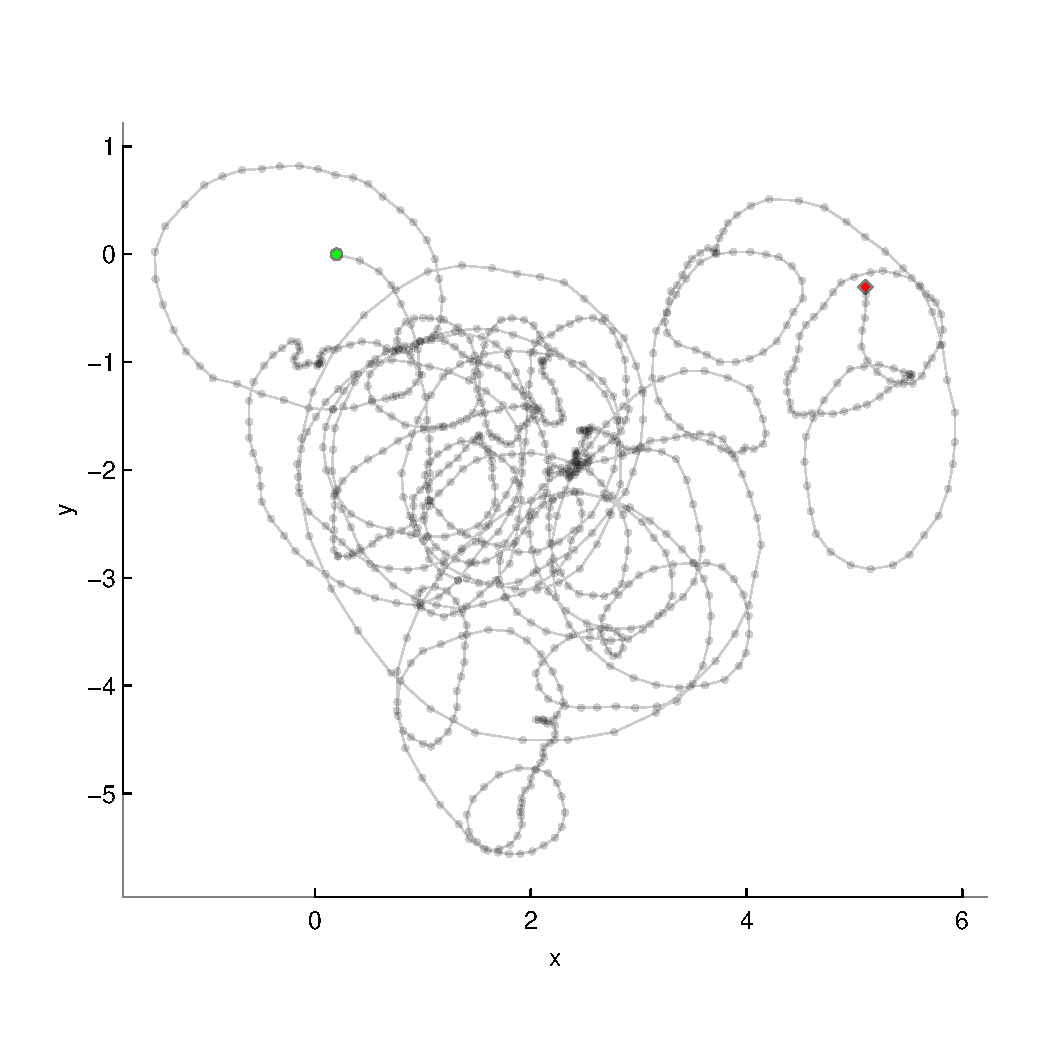
\includegraphics[width=\maxwidth]{figure/rcvm-1} 

\end{knitrout}
   \end{minipage}
  \begin{minipage}{0.6\linewidth}
\begin{knitrout}\small
\definecolor{shadecolor}{rgb}{0.969, 0.969, 0.969}\color{fgcolor}\begin{kframe}
\begin{alltt}
\hlkwd{with}\hlstd{(rcvm,} \hlkwd{estimateRACVM}\hlstd{(}\hlkwc{Z}\hlstd{=Z,} \hlkwc{T}\hlstd{=T,} \hlkwc{model} \hlstd{=} \hlstr{"RCVM"}\hlstd{,}
                         \hlkwc{compare.models}\hlstd{=}\hlnum{TRUE}\hlstd{))}
\end{alltt}
\begin{verbatim}
## $results
##               eta    omega      tau      rms
## Estimate 2.107711 1.911959 5.418521 2.107711
## CI.low   1.613949 1.824789 3.376816 1.613949
## CI.high  2.601473 1.999128 8.694689 2.601473
## 
## $LL
## [1] -317.9043
## 
## $CompareTable
##         logLike k       AIC     deltaAIC       BIC   deltaBIC
## UCVM  -985.7452 2 1975.4905 1333.6818179 1985.3060 1328.77406
## ACVM  -985.7236 4 1979.4471 1337.6384656 1999.0782 1342.54622
## RCVM  -317.9043 3  641.8087    0.0000000  656.5319    0.00000
## RACVM -316.3394 5  642.6787    0.8700291  667.2175   10.68554
\end{verbatim}
\end{kframe}
\end{knitrout}
     \end{minipage}


\subsubsection{Rotational-Advective CVM}
     \begin{minipage}{0.4\linewidth}   
  \noindent
\begin{knitrout}
\definecolor{shadecolor}{rgb}{0.969, 0.969, 0.969}\color{fgcolor}
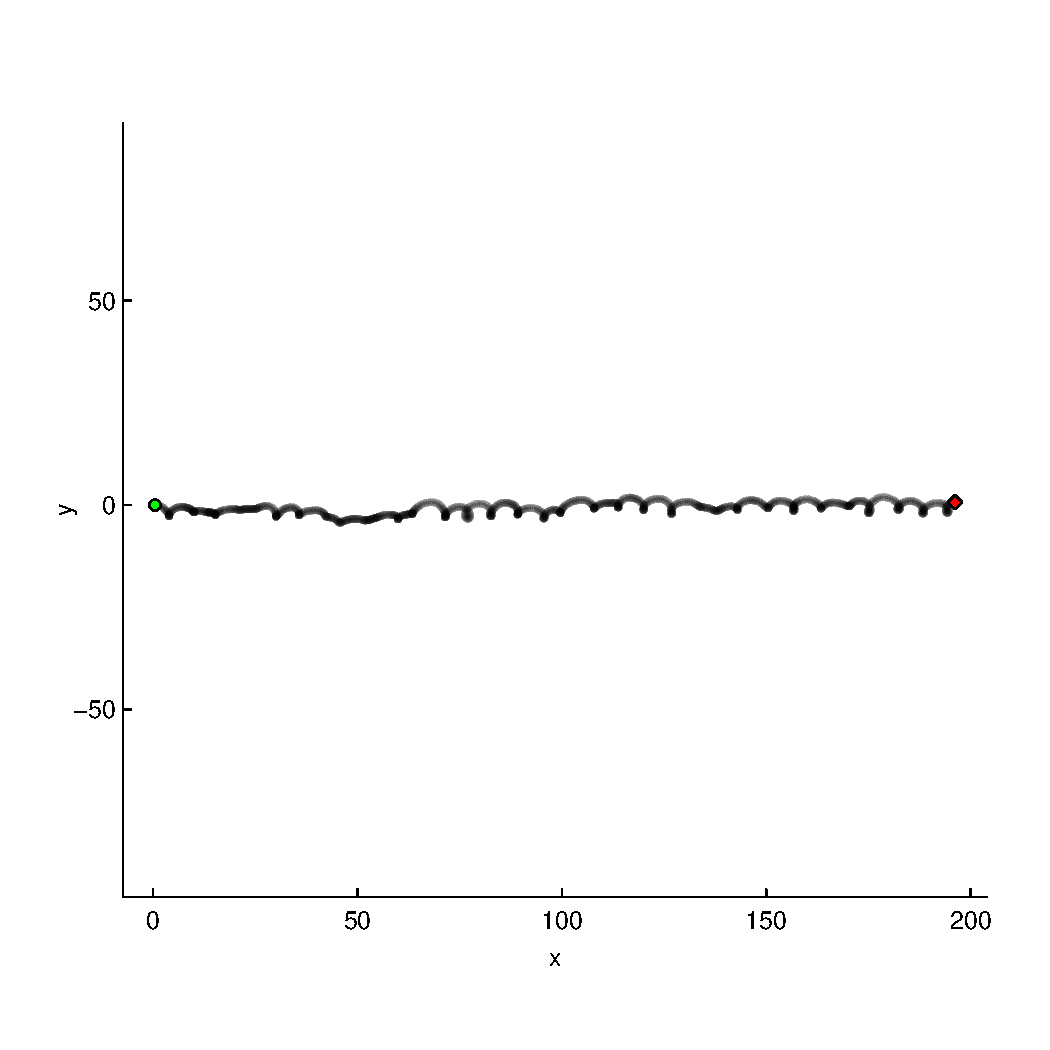
\includegraphics[width=\maxwidth]{figure/racvm-1} 

\end{knitrout}
   \end{minipage}
  \begin{minipage}{0.6\linewidth}
\begin{knitrout}\footnotesize
\definecolor{shadecolor}{rgb}{0.969, 0.969, 0.969}\color{fgcolor}\begin{kframe}
\begin{alltt}
\hlkwd{with}\hlstd{(racvm,} \hlkwd{estimateRACVM}\hlstd{(}\hlkwc{Z}\hlstd{=Z,} \hlkwc{T}\hlstd{=T,} \hlkwc{model} \hlstd{=} \hlstr{"RACVM"}\hlstd{,}
                          \hlkwc{compare.models}\hlstd{=}\hlnum{TRUE}\hlstd{))}
\end{alltt}
\begin{verbatim}
## $results
##               eta    omega     mu.x         mu.y       tau      rms
## Estimate 2.683952 1.957792 1.914226  0.006262927  8.871261 3.304948
## CI.low   1.908777 1.876463 1.822127 -0.085867701  4.952038 2.672787
## CI.high  3.459126 2.039121 2.006324  0.098393556 15.892301 3.937109
## 
## $LL
## [1] -331.6268
## 
## $CompareTable
##          logLike k       AIC  deltaAIC       BIC  deltaBIC
## UCVM  -1085.4011 2 2174.8021 1501.5486 2184.6177 1486.8253
## ACVM  -1078.4676 4 2164.9353 1491.6817 2184.5663 1486.7740
## RCVM   -725.9937 3 1457.9873  784.7338 1472.7106  774.9182
## RACVM  -331.6268 5  673.2536    0.0000  697.7923    0.0000
\end{verbatim}
\end{kframe}
\end{knitrout}
     \end{minipage}

Note that the results of these fits also report the root mean squared (\emph{rms}) speed.  This is a derived quantity equal to:
$$rms = \sqrt{\eta^2 + \mu_x^2 +\mu_y^2}$$
\noindent For unbiased CVM's, it is simple equal to $\eta$. The rms speed is useful for comparing across advective and non-advective models.  There are some technical nuances to computing the confidence intervals around the rms (see Appendix). 

\subsection{Kestrel data}

In the paper, we analyze a phenomenal data set of a single lesser kestrel (\emph{Falco naumanni}) flight in southern Spain from Hern{\'a}ndez-Pliego et al (2015a, 2015b). One kestrel's flight is in the package:

\begin{knitrout}
\definecolor{shadecolor}{rgb}{0.969, 0.969, 0.969}\color{fgcolor}\begin{kframe}
\begin{alltt}
\hlkwd{data}\hlstd{(Kestrel);} \hlkwd{plot_track}\hlstd{(Kestrel[,}\hlkwd{c}\hlstd{(}\hlstr{"X"}\hlstd{,}\hlstr{"Y"}\hlstd{)],} \hlkwc{cex}\hlstd{=}\hlnum{0.3}\hlstd{)}
\end{alltt}
\end{kframe}

{\centering 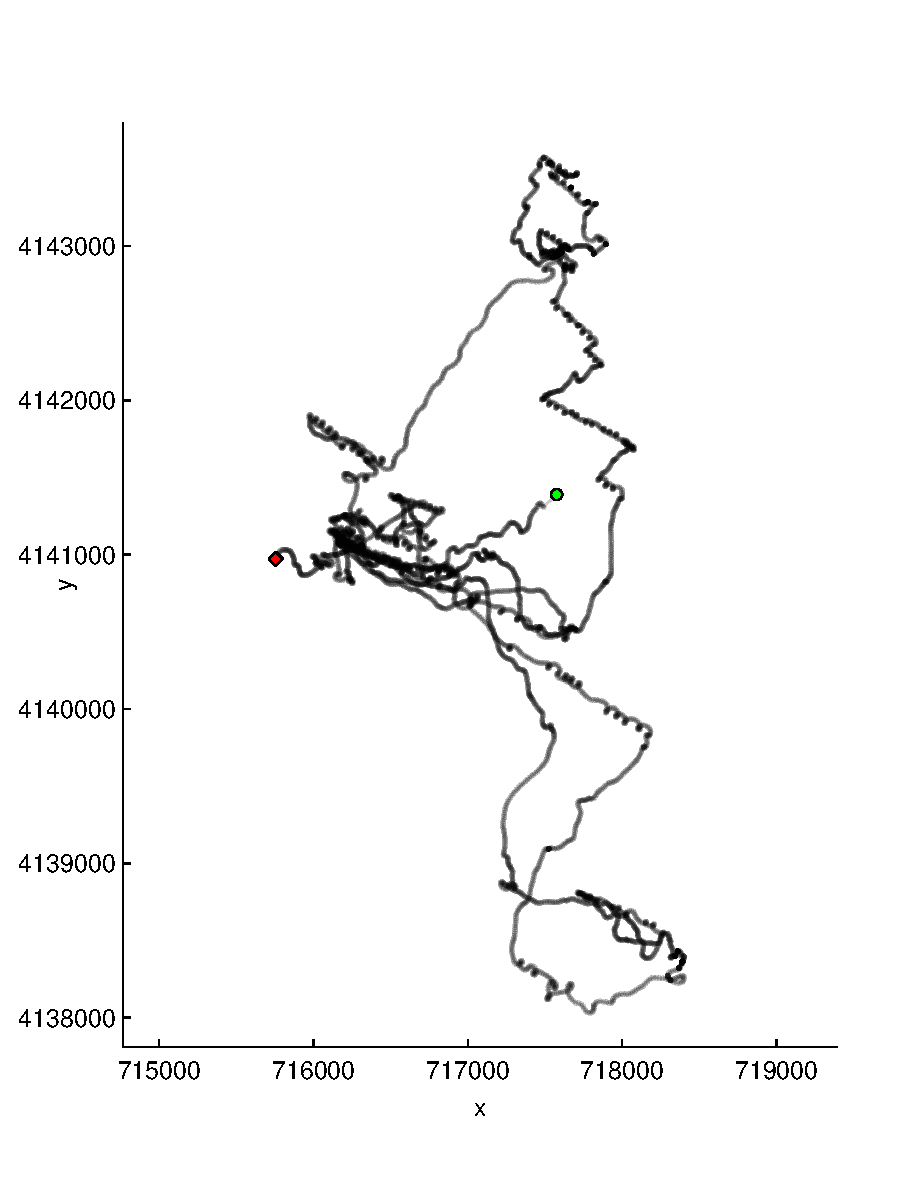
\includegraphics[width=3in]{figure/KestrelFlight-1} 

}



\end{knitrout}


\noindent We can analyze one portions of the kestrel's flight, mirroring the analysis in Gurarie (in review).  The following 90 second snippet is clearly advective and rotational:

\begin{knitrout}
\definecolor{shadecolor}{rgb}{0.969, 0.969, 0.969}\color{fgcolor}\begin{kframe}
\begin{alltt}
  \hlstd{K1} \hlkwb{<-} \hlstd{Kestrel[}\hlnum{3360}\hlopt{:}\hlnum{3450}\hlstd{,]}
  \hlkwd{with}\hlstd{(K1,} \hlkwd{scan_track}\hlstd{(}\hlkwc{x}\hlstd{=X,} \hlkwc{y}\hlstd{=Y))}
\end{alltt}
\end{kframe}
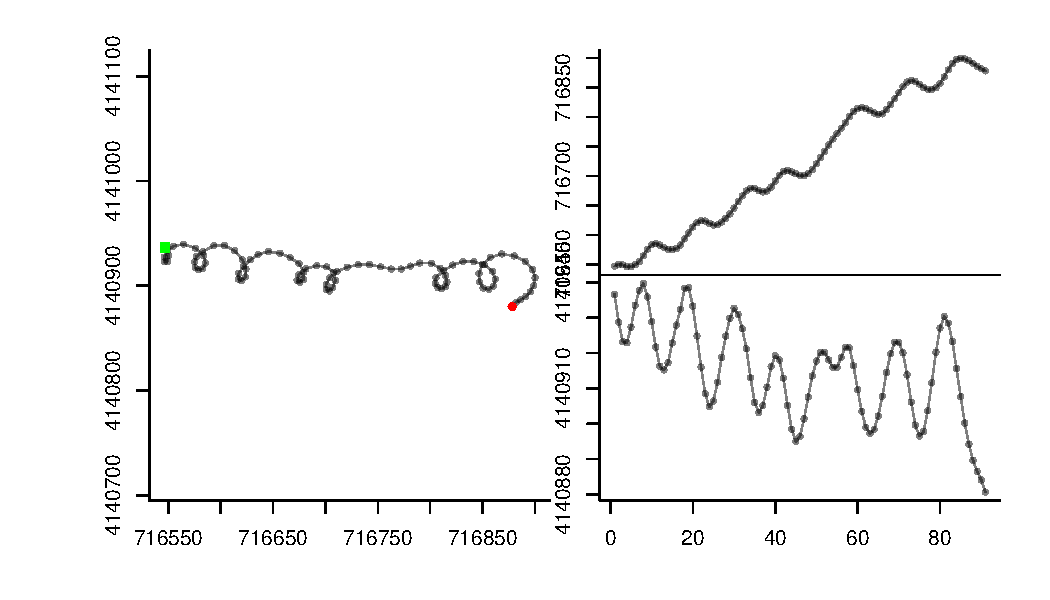
\includegraphics[width=\maxwidth]{figure/K1-1} 

\end{knitrout}

\noindent The model selection confirms this (note that we specify the time unit of analysis - in this case, seconds).

\begin{knitrout}
\definecolor{shadecolor}{rgb}{0.969, 0.969, 0.969}\color{fgcolor}\begin{kframe}
\begin{alltt}
\hlstd{(fit1} \hlkwb{<-} \hlkwd{with}\hlstd{(K1,} \hlkwd{estimateRACVM}\hlstd{(}\hlkwc{XY} \hlstd{=} \hlkwd{cbind}\hlstd{(X,Y),} \hlkwc{T} \hlstd{= timestamp,} \hlkwc{spline}\hlstd{=}\hlnum{TRUE}\hlstd{,}
                                \hlkwc{model} \hlstd{=} \hlstr{"RACVM"}\hlstd{,} \hlkwc{time.units} \hlstd{=} \hlstr{"sec"}\hlstd{)))}
\end{alltt}
\begin{verbatim}
## $results
##                eta     omega     mu.x       mu.y        tau       rms
## Estimate  7.588318 0.5088868 3.867659 -0.3625973  31.508582  8.605233
## CI.low    3.044545 0.4702505 3.299105 -0.9311530   9.331182  4.606687
## CI.high  12.132090 0.5475230 4.436212  0.2059585 106.394962 12.603779
## 
## $LL
## [1] -303.429
## 
## $CompareTable
##         logLike k      AIC deltaAIC      BIC  deltaBIC
## UCVM  -439.6961 2 883.3922 266.5342 888.3918 259.03478
## ACVM  -438.7136 4 885.4271 268.5691 895.4263 266.06930
## RCVM  -357.2247 3 720.4495 103.5915 727.9489  98.59185
## RACVM -303.4290 5 616.8580   0.0000 629.3570   0.00000
\end{verbatim}
\end{kframe}
\end{knitrout}

\noindent  The track is very regularly but very slightly coarsely sampled.  We therefore use the spline correction (though its impact is probably minimal).  The model selection strongly prefers an RACVM model.  The rotational speed is about 0.5 radians per second, the advective speed is around 4 m/sec. We feed these estimates back into the simulation algorithm to simulate a trajectory:  

\begin{knitrout}
\definecolor{shadecolor}{rgb}{0.969, 0.969, 0.969}\color{fgcolor}\begin{kframe}
\begin{alltt}
\hlstd{p.fit1} \hlkwb{<-} \hlkwd{with}\hlstd{(fit1}\hlopt{$}\hlstd{results,} \hlkwd{list}\hlstd{(}\hlkwc{eta}\hlstd{=eta[}\hlnum{1}\hlstd{],} \hlkwc{tau} \hlstd{= tau[}\hlnum{1}\hlstd{],}
                                  \hlkwc{mu} \hlstd{= mu.x[}\hlnum{1}\hlstd{]} \hlopt{+} \hlnum{1i}\hlopt{*}\hlstd{mu.y[}\hlnum{1}\hlstd{],}
                                  \hlkwc{omega} \hlstd{= omega[}\hlnum{1}\hlstd{],} \hlkwc{v0} \hlstd{=} \hlkwd{diff}\hlstd{(K1}\hlopt{$}\hlstd{Z)[}\hlnum{1}\hlstd{]))}
\hlstd{K1.sim} \hlkwb{<-} \hlkwd{with}\hlstd{(p.fit1,} \hlkwd{simulateRACVM}\hlstd{(}\hlkwc{eta}\hlstd{=eta,} \hlkwc{tau}\hlstd{=tau,} \hlkwc{mu} \hlstd{= mu,} \hlkwc{omega}\hlstd{=omega,}
                                     \hlkwc{Tmax} \hlstd{=} \hlkwd{nrow}\hlstd{(K1),} \hlkwc{v0} \hlstd{= v0,} \hlkwc{dt} \hlstd{=} \hlnum{1}\hlstd{))}
\hlkwd{with}\hlstd{(K1.sim,} \hlkwd{scan_track}\hlstd{(}\hlkwc{z}\hlstd{=Z))}
\end{alltt}
\end{kframe}
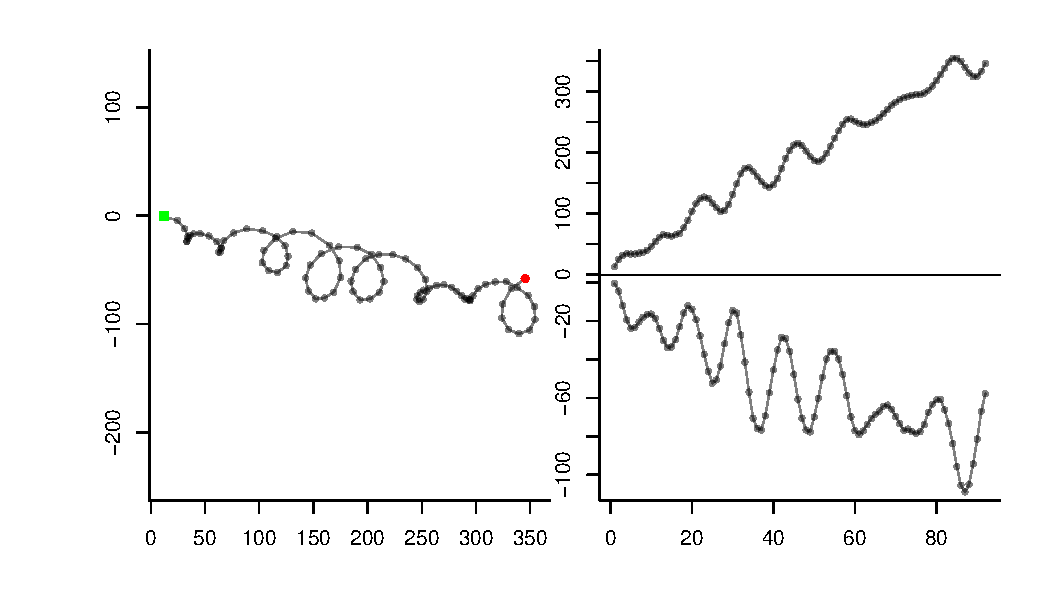
\includegraphics[width=\maxwidth]{figure/K1_sim-1} 

\end{knitrout}
\noindent Visually, the simulation looks rather similar to the data snippet with respect to radii and frequency of rotations, randomness and advective tendency.  


\section{Behavioral change point analyses}

Change point analysis (like most of ecological analysis) is not an exact science.  However, the existence of likelihoods and model selection criteria makes it possible to develop an heuristic that can propose and assess candidate change points, select ``significant'' ones, and estimate the movement model and parameters between those change points.  

\subsection{Identifying a single change point}

Simulate a two-phase UCVM:

\begin{knitrout}
\definecolor{shadecolor}{rgb}{0.969, 0.969, 0.969}\color{fgcolor}\begin{kframe}
\begin{alltt}
\hlstd{ucvm1} \hlkwb{<-} \hlkwd{simulateUCVM}\hlstd{(}\hlkwc{T}\hlstd{=}\hlkwd{cumsum}\hlstd{(}\hlkwd{rexp}\hlstd{(}\hlnum{100}\hlstd{)),} \hlkwc{nu}\hlstd{=}\hlnum{2}\hlstd{,} \hlkwc{tau}\hlstd{=}\hlnum{1}\hlstd{,} \hlkwc{method}\hlstd{=}\hlstr{"exact"}\hlstd{)}
\hlstd{ucvm2} \hlkwb{<-} \hlkwd{simulateUCVM}\hlstd{(}\hlkwc{T}\hlstd{=}\hlkwd{cumsum}\hlstd{(}\hlkwd{rexp}\hlstd{(}\hlnum{100}\hlstd{)),} \hlkwc{nu}\hlstd{=}\hlnum{2}\hlstd{,} \hlkwc{tau}\hlstd{=}\hlnum{10}\hlstd{,} \hlkwc{v0} \hlstd{= ucvm1}\hlopt{$}\hlstd{V[}\hlnum{100}\hlstd{],} \hlkwc{method}\hlstd{=}\hlstr{"exact"}\hlstd{)}
\hlstd{T} \hlkwb{<-} \hlkwd{c}\hlstd{(ucvm1}\hlopt{$}\hlstd{T, ucvm1}\hlopt{$}\hlstd{T[}\hlnum{100}\hlstd{]} \hlopt{+} \hlstd{ucvm2}\hlopt{$}\hlstd{T)}
\hlstd{Z} \hlkwb{<-} \hlkwd{c}\hlstd{(ucvm1}\hlopt{$}\hlstd{Z, ucvm1}\hlopt{$}\hlstd{Z[}\hlnum{100}\hlstd{]} \hlopt{+} \hlstd{ucvm2}\hlopt{$}\hlstd{Z)}
\hlkwd{plot_track}\hlstd{(Z)}
\end{alltt}
\end{kframe}

{\centering 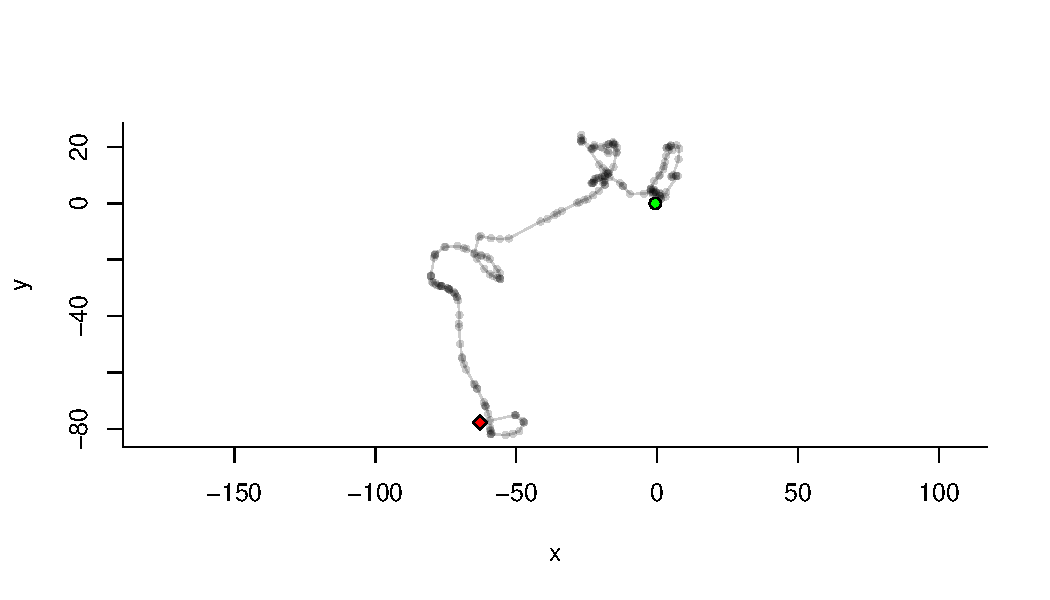
\includegraphics[width=6in]{figure/TwoPhaseCVM-1} 

}



\end{knitrout}

\noindent The only parameter that changed in this simulation is the time scale - it is not necessarily easy to identify by eye where the model switched. The likelihood of all candidate change points within this track is found using the \texttt{findSingleBreakPoint} as follows:

\begin{knitrout}
\definecolor{shadecolor}{rgb}{0.969, 0.969, 0.969}\color{fgcolor}\begin{kframe}
\begin{alltt}
\hlkwd{findSingleBreakPoint}\hlstd{(Z,T,} \hlkwc{method} \hlstd{=} \hlstr{"sweep"}\hlstd{)}
\end{alltt}
\end{kframe}
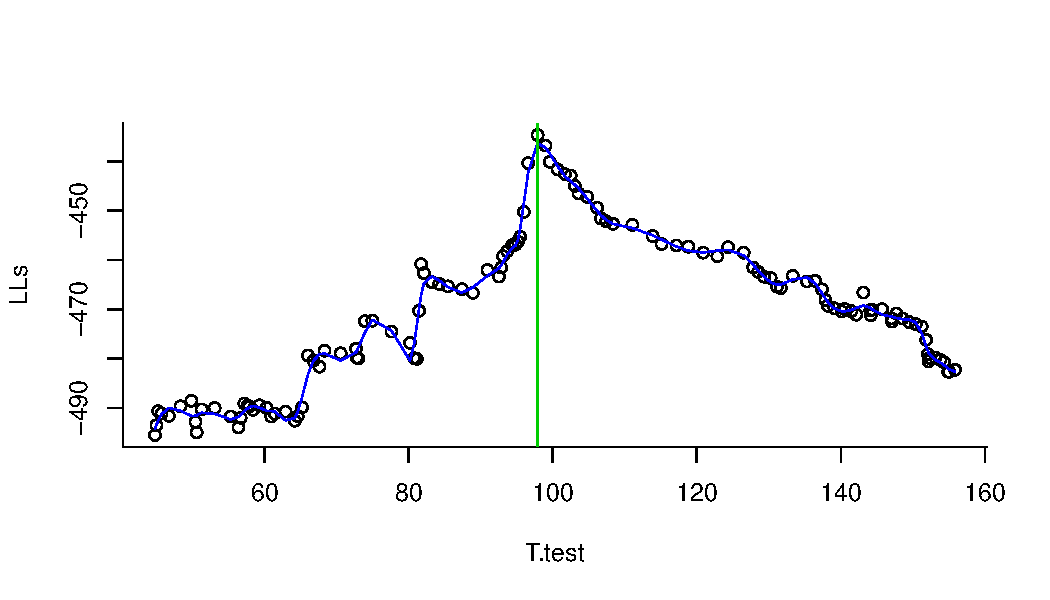
\includegraphics[width=\maxwidth]{figure/unnamed-chunk-11-1} 
\begin{kframe}\begin{verbatim}
## [1] 107.554
\end{verbatim}
\end{kframe}
\end{knitrout}

This is a good estimate of the true change point, which occurred at time 106.3219321.

Note, this function only works on the UCVM model - i.e.~it is useful for identifying sudden changes in time scales $\tau$ and rms speeds $\eta$ for unbiased movements only. 


\subsection{Multiple change points}

To find multiple change points where the number of changes is unknown \emph{a priori} AND the underlying model changes, we follow these steps:
\begin{enumerate}
\item  sweep a change point analysis window across the entire time series to obtain \emph{candidate change points}.   
\item separately assess the ``significance'' of each of the change points with respect to both parameters and movement model selection, iteratively removing non-significant changepoints and re-assessing
\item estimate the final models and parameter values within the final selected set of phases.
\end{enumerate}

We perform an example of this analysis on a simulated trajectory with 3 behavioral phases, switching from an advective, fairly high speed movement, to an unbiased, moderately fast movement, to a highly uncorrelated slower movement. Roughly, this might approximate the shifts between commuting to a foraging site, switching to a searching behavior, and switching to an intensive foraging behavior.  

\begin{knitrout}
\definecolor{shadecolor}{rgb}{0.969, 0.969, 0.969}\color{fgcolor}\begin{kframe}
\begin{alltt}
\hlstd{taus} \hlkwb{<-} \hlkwd{c}\hlstd{(}\hlnum{3}\hlstd{,} \hlnum{3}\hlstd{,} \hlnum{1}\hlstd{)}
\hlstd{mus} \hlkwb{<-} \hlkwd{c}\hlstd{(}\hlnum{2}\hlstd{,} \hlnum{0}\hlstd{,} \hlnum{0}\hlstd{)}
\hlstd{etas} \hlkwb{<-} \hlkwd{c}\hlstd{(}\hlnum{2}\hlstd{,} \hlnum{1}\hlstd{,} \hlnum{1}\hlstd{)}
\hlstd{durations} \hlkwb{<-} \hlkwd{c}\hlstd{(}\hlnum{40}\hlstd{,}\hlnum{60}\hlstd{,}\hlnum{100}\hlstd{)}

\hlstd{Z.raw} \hlkwb{<-} \hlnum{0}
\hlstd{T.raw} \hlkwb{<-} \hlnum{0}
\hlstd{mycvm} \hlkwb{<-} \hlkwd{list}\hlstd{()}

\hlkwa{for}\hlstd{(i} \hlkwa{in} \hlnum{1}\hlopt{:}\hlkwd{length}\hlstd{(taus))\{}
  \hlkwa{if}\hlstd{(i} \hlopt{>} \hlnum{1}\hlstd{)  v0} \hlkwb{<-} \hlstd{mycvm}\hlopt{$}\hlstd{V[}\hlkwd{length}\hlstd{(mycvm)]}  \hlkwa{else} \hlstd{v0} \hlkwb{=} \hlstd{mus[}\hlnum{1}\hlstd{]}
  \hlstd{mycvm} \hlkwb{<-} \hlkwd{simulateRACVM}\hlstd{(}\hlkwc{tau} \hlstd{= taus[i],} \hlkwc{eta} \hlstd{= etas[i],} \hlkwc{mu} \hlstd{= mus[i],} \hlkwc{v0} \hlstd{= v0,}
                         \hlkwc{Tmax} \hlstd{= durations[i],} \hlkwc{dt} \hlstd{=} \hlnum{0.01}\hlstd{)}
  \hlstd{Z.raw} \hlkwb{<-} \hlkwd{c}\hlstd{(Z.raw, mycvm}\hlopt{$}\hlstd{Z} \hlopt{+} \hlstd{Z.raw[}\hlkwd{length}\hlstd{(Z.raw)])}
  \hlstd{T.raw} \hlkwb{<-} \hlkwd{c}\hlstd{(T.raw, mycvm}\hlopt{$}\hlstd{T} \hlopt{+} \hlstd{T.raw[}\hlkwd{length}\hlstd{(T.raw)])}
\hlstd{\}}
\end{alltt}
\end{kframe}
\end{knitrout}

For the analysis, we will randomly sample 400 observations from the complete data:

\begin{knitrout}
\definecolor{shadecolor}{rgb}{0.969, 0.969, 0.969}\color{fgcolor}\begin{kframe}
\begin{alltt}
\hlkwd{par}\hlstd{(}\hlkwc{bty} \hlstd{=} \hlstr{"l"}\hlstd{,} \hlkwc{mar} \hlstd{=} \hlkwd{c}\hlstd{(}\hlnum{0}\hlstd{,}\hlnum{4}\hlstd{,}\hlnum{0}\hlstd{,}\hlnum{0}\hlstd{),} \hlkwc{oma} \hlstd{=} \hlkwd{c}\hlstd{(}\hlnum{4}\hlstd{,}\hlnum{0}\hlstd{,}\hlnum{2}\hlstd{,}\hlnum{2}\hlstd{),} \hlkwc{xpd} \hlstd{=} \hlnum{NA}\hlstd{)}
\hlstd{multicvm} \hlkwb{<-} \hlkwd{data.frame}\hlstd{(}\hlkwc{Z} \hlstd{= Z.raw,} \hlkwc{T} \hlstd{= T.raw)[}\hlkwd{sample}\hlstd{(}\hlnum{1}\hlopt{:}\hlkwd{length}\hlstd{(Z.raw),} \hlnum{400}\hlstd{),]} \hlopt \hlkwd{arrange}\hlstd{(T)}
\hlkwd{with}\hlstd{(multicvm,} \hlkwd{scan_track}\hlstd{(}\hlkwc{z} \hlstd{= Z,} \hlkwc{time} \hlstd{= T))}
\end{alltt}
\end{kframe}
\includegraphics[width=\maxwidth]{figure/plotMulticvm__echo_-1-1} 

\end{knitrout}

\noindent The actual change points occur at times 40 and  100.

\subsubsection{Step I - the Window Sweep} 

To perform a window sweep, we need to set two variables: the \emph{windowsize} of analysis and the \emph{windowstep}.  Both are set in units of time.  The window size is the temporal interval of analysis, the step is the increment by which the analysis windows are moved forward.

Setting the analysis window size is totally the user's choice. The size should be driven by biological considerations. Ideally, it will be large enough to encompass one, but not two or more change points.  The smaller the window step, the more ``thorough'' the analysis, but ultimately its size is not very important as long as it is much smaller than the analysis window.  Ultimately, for strong changes, the analysis will not be very sensitive to reasonable values of either of these parameters.  

Note that if there are gaps in the data or they are irregular, the data extent of the window will be smaller, and if there are fewer than 30 data points in the window, the window will be skipped.  Note also, that the window sweep is only working with a single model which should be specified. It should be the most complex model you are interested (in our case, the ACVM).   

\begin{knitrout}
\definecolor{shadecolor}{rgb}{0.969, 0.969, 0.969}\color{fgcolor}\begin{kframe}
\begin{alltt}
\hlstd{Z} \hlkwb{<-} \hlstd{multicvm}\hlopt{$}\hlstd{Z}
\hlstd{T} \hlkwb{<-} \hlstd{multicvm}\hlopt{$}\hlstd{T}
\hlstd{simSweep} \hlkwb{<-} \hlkwd{sweepRACVM}\hlstd{(}\hlkwc{Z}\hlstd{=Z,} \hlkwc{T}\hlstd{=T,} \hlkwc{windowsize} \hlstd{=} \hlnum{80}\hlstd{,} \hlkwc{windowstep} \hlstd{=} \hlnum{5}\hlstd{,} \hlkwc{model} \hlstd{=} \hlstr{"ACVM"}\hlstd{,} \hlkwc{progress}\hlstd{=}\hlnum{FALSE}\hlstd{)}
\end{alltt}
\end{kframe}
\end{knitrout}

\noindent Toggling the \texttt{progress} to TRUE will provide reports on the progress of the analysis.  There is also an option to parallelize the analysis using the \texttt{doParallel} and \texttt{foreach} R packages.  This which can speed things up considerably (roughly in proportion to the number of cores on your processor).  An example of implementation: 

\begin{knitrout}
\definecolor{shadecolor}{rgb}{0.969, 0.969, 0.969}\color{fgcolor}\begin{kframe}
\begin{alltt}
\hlkwd{require}\hlstd{(foreach);} \hlkwd{require}\hlstd{(doParallel)}
\hlstd{cl} \hlkwb{<-} \hlkwd{makeCluster}\hlstd{(}\hlkwd{detectCores}\hlstd{())}
\hlkwd{registerDoParallel}\hlstd{(cl)}
\hlstd{simSweep} \hlkwb{<-} \hlkwd{sweepRACVM}\hlstd{(}\hlkwc{Z}\hlstd{=Z,} \hlkwc{T}\hlstd{=T,} \hlkwc{windowsize} \hlstd{=} \hlnum{80}\hlstd{,} \hlkwc{windowstep} \hlstd{=} \hlnum{5}\hlstd{,} \hlkwc{model} \hlstd{=} \hlstr{"ACVM"}\hlstd{,} \hlkwc{.parallel} \hlstd{=} \hlnum{TRUE}\hlstd{)}
\end{alltt}
\end{kframe}
\end{knitrout}



This function outputs a jagged matrix of likelihood estimates, which can be visualized: 

\begin{knitrout}
\definecolor{shadecolor}{rgb}{0.969, 0.969, 0.969}\color{fgcolor}\begin{kframe}
\begin{alltt}
\hlkwd{plotWindowSweep}\hlstd{(simSweep)}
\end{alltt}
\end{kframe}
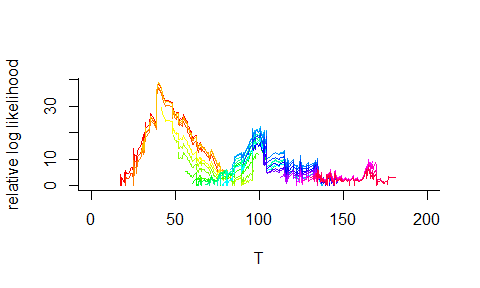
\includegraphics[width=\maxwidth]{figure/loadsimSweep-1} 

\end{knitrout}

\noindent In the image above, each color represents the relative log-likelihood profile for a single window. There are two very distinct peaks, the remainder of the algorithm boils these down to ``significant'' change points. 

\subsubsection{Step II - Obtain Candidate Change Points} 

We obtain candidate change points by taking all of the most likely change points (MLCP) in each of the windows, listing all of the MLCP's.  The function that does this is \texttt{findCandidateChangePoints}.  Here is a complete list of candidates:

\begin{knitrout}
\definecolor{shadecolor}{rgb}{0.969, 0.969, 0.969}\color{fgcolor}\begin{kframe}
\begin{alltt}
\hlstd{CP.all} \hlkwb{<-} \hlkwd{findCandidateChangePoints}\hlstd{(}\hlkwc{windowsweep} \hlstd{= simSweep,} \hlkwc{clusterwidth} \hlstd{=} \hlnum{0}\hlstd{)}
\end{alltt}


{\ttfamily\noindent\itshape\color{messagecolor}{\#\# Note: clustering candidate change points at 0 time units collapsed 6 candidate change points to 6 change points.}}

{\ttfamily\noindent\color{warningcolor}{\#\# Warning in findCandidateChangePoints(windowsweep = simSweep, clusterwidth = 0): \\\#\#\ \ Some of your partitions are very small - probably too small. You might consider re-clustering the change points with a threshold of at least 0.61.}}\begin{alltt}
\hlkwd{str}\hlstd{(CP.all)}
\end{alltt}
\begin{verbatim}
##  atomic [1:6] 40 45.1 99.4 100 116.9 ...
##  - attr(*, "time.unit")= chr "auto"
##  - attr(*, "time")= num [1:400] 0.48 0.69 1.12 1.68 2.26 3 3.57 4.04 4.13 4.91 ...
\end{verbatim}
\end{kframe}
\end{knitrout}

\noindent The warning lets us know that some of the candidate change points are rather too close (in time) to each other, and it might be a good idea to cluster them, i.e.~assign multiple points within a given time interval to a single cluster. If we take a rather generous cluster width below: 

\begin{knitrout}
\definecolor{shadecolor}{rgb}{0.969, 0.969, 0.969}\color{fgcolor}\begin{kframe}
\begin{alltt}
\hlstd{CP.clustered} \hlkwb{<-} \hlkwd{findCandidateChangePoints}\hlstd{(}\hlkwc{windowsweep} \hlstd{= simSweep,} \hlkwc{clusterwidth} \hlstd{=} \hlnum{4}\hlstd{)}
\end{alltt}


{\ttfamily\noindent\itshape\color{messagecolor}{\#\# Note: clustering candidate change points at 4 time units collapsed 6 candidate change points to 5 change points.}}\begin{alltt}
\hlkwd{str}\hlstd{(CP.clustered)}
\end{alltt}
\begin{verbatim}
##  atomic [1:5] 40 45.1 99.7 116.9 157.1
##  - attr(*, "time.unit")= chr "auto"
##  - attr(*, "time")= num [1:400] 0.48 0.69 1.12 1.68 2.26 3 3.57 4.04 4.13 4.91 ...
\end{verbatim}
\end{kframe}
\end{knitrout}

\noindent We now have a somewhat smaller set of change points to assess.  

\subsubsection{Step III - Selecting Significant Change Points}  

We use the set of candidate change points to separate the track into phases and for each change point (i.e.~pair of neighboring phases) we assess the ``significance'' of the change point by comparing the BIC (or AIC) of a two-model versus one-model fit.  The function that performs this is \texttt{getCPtable}

\begin{knitrout}
\definecolor{shadecolor}{rgb}{0.969, 0.969, 0.969}\color{fgcolor}\begin{kframe}
\begin{alltt}
\hlkwd{getCPtable}\hlstd{(}\hlkwc{CPs} \hlstd{= CP.clustered,} \hlkwc{Z} \hlstd{= Z,} \hlkwc{T} \hlstd{= T,} \hlkwc{modelset} \hlstd{=} \hlkwd{c}\hlstd{(}\hlstr{"UCVM"}\hlstd{,} \hlstr{"ACVM"}\hlstd{),} \hlkwc{tidy} \hlstd{=} \hlkwa{NULL}\hlstd{)}
\end{alltt}


{\ttfamily\noindent\color{warningcolor}{\#\# Warning in min(i1): no non-missing arguments to min; returning Inf}}

{\ttfamily\noindent\color{warningcolor}{\#\# Warning in max(i2): no non-missing arguments to max; returning -Inf}}

{\ttfamily\noindent\bfseries\color{errorcolor}{\#\# Error in min(i1):max(i2): result would be too long a vector}}\end{kframe}
\end{knitrout}

\noindent In the output of \texttt{selectRACVM}, the \texttt{extremes} column indicates which parameter showed significant changes in parameter values defined by no overlap in the 95\% confidence interval, and the \texttt{dAIC} and \texttt{dBIC} compare the change point model to the no change point model.  We can ask this function to tidy the selection table according to any combination of several criteria: - by the differences, or by negative dAIC or dBIC, or by a mismatch in the models selected (see the help file). 

\begin{knitrout}
\definecolor{shadecolor}{rgb}{0.969, 0.969, 0.969}\color{fgcolor}\begin{kframe}
\begin{alltt}
\hlkwd{getCPtable}\hlstd{(}\hlkwc{CPs} \hlstd{= CP.clustered,} \hlkwc{Z} \hlstd{= Z,} \hlkwc{T} \hlstd{= T,} \hlkwc{modelset} \hlstd{=} \hlkwd{c}\hlstd{(}\hlstr{"UCVM"}\hlstd{,} \hlstr{"ACVM"}\hlstd{),}  \hlkwc{iterate} \hlstd{=} \hlnum{TRUE}\hlstd{)}
\end{alltt}


{\ttfamily\noindent\color{warningcolor}{\#\# Warning in min(i1): no non-missing arguments to min; returning Inf}}

{\ttfamily\noindent\color{warningcolor}{\#\# Warning in max(i2): no non-missing arguments to max; returning -Inf}}

{\ttfamily\noindent\bfseries\color{errorcolor}{\#\# Error in min(i1):max(i2): result would be too long a vector}}\end{kframe}
\end{knitrout}

\noindent We now have a final selected set of change points and, perhaps more usefully, a summary of which parameters precisely changed.  Note that thanks to the magic of \texttt{magrittr} piping, the process of finding and selecting change points can be reduced to a single line of code, which is convenient for comparing the robustness of the different settings.  Replicating the above analysis for several cluster widths yield the same result:

\begin{knitrout}
\definecolor{shadecolor}{rgb}{0.969, 0.969, 0.969}\color{fgcolor}\begin{kframe}
\begin{alltt}
\hlstd{simSweep} \hlopt \hlkwd{findCandidateChangePoints}\hlstd{(}\hlkwc{clusterwidth} \hlstd{=} \hlnum{2}\hlstd{)} \hlopt
  \hlkwd{getCPtable}\hlstd{(}\hlkwc{Z} \hlstd{= Z,} \hlkwc{T} \hlstd{= T,} \hlkwc{modelset} \hlstd{=} \hlkwd{c}\hlstd{(}\hlstr{"UCVM"}\hlstd{,} \hlstr{"ACVM"}\hlstd{))}
\end{alltt}


{\ttfamily\noindent\itshape\color{messagecolor}{\#\# Note: clustering candidate change points at 2 time units collapsed 6 candidate change points to 5 change points.}}

{\ttfamily\noindent\color{warningcolor}{\#\# Warning in min(i1): no non-missing arguments to min; returning Inf}}

{\ttfamily\noindent\color{warningcolor}{\#\# Warning in max(i2): no non-missing arguments to max; returning -Inf}}

{\ttfamily\noindent\bfseries\color{errorcolor}{\#\# Error in min(i1):max(i2): result would be too long a vector}}\begin{alltt}
\hlstd{simSweep} \hlopt \hlkwd{findCandidateChangePoints}\hlstd{(}\hlkwc{clusterwidth} \hlstd{=} \hlnum{4}\hlstd{)} \hlopt
  \hlkwd{getCPtable}\hlstd{(}\hlkwc{Z} \hlstd{= Z,} \hlkwc{T} \hlstd{= T,} \hlkwc{modelset} \hlstd{=} \hlkwd{c}\hlstd{(}\hlstr{"UCVM"}\hlstd{,} \hlstr{"ACVM"}\hlstd{))}
\end{alltt}


{\ttfamily\noindent\itshape\color{messagecolor}{\#\# Note: clustering candidate change points at 4 time units collapsed 6 candidate change points to 5 change points.}}

{\ttfamily\noindent\color{warningcolor}{\#\# Warning in min(i1): no non-missing arguments to min; returning Inf}}

{\ttfamily\noindent\color{warningcolor}{\#\# Warning in min(i1): no non-missing arguments to max; returning -Inf}}

{\ttfamily\noindent\bfseries\color{errorcolor}{\#\# Error in min(i1):max(i2): result would be too long a vector}}\begin{alltt}
\hlstd{simSweep} \hlopt \hlkwd{findCandidateChangePoints}\hlstd{(}\hlkwc{clusterwidth} \hlstd{=} \hlnum{10}\hlstd{)} \hlopt
  \hlkwd{getCPtable}\hlstd{(}\hlkwc{Z} \hlstd{= Z,} \hlkwc{T} \hlstd{= T,} \hlkwc{modelset} \hlstd{=} \hlkwd{c}\hlstd{(}\hlstr{"UCVM"}\hlstd{,} \hlstr{"ACVM"}\hlstd{))}
\end{alltt}


{\ttfamily\noindent\itshape\color{messagecolor}{\#\# Note: clustering candidate change points at 10 time units collapsed 6 candidate change points to 4 change points.}}

{\ttfamily\noindent\color{warningcolor}{\#\# Warning in min(i1): no non-missing arguments to min; returning Inf}}

{\ttfamily\noindent\color{warningcolor}{\#\# Warning in min(i1): no non-missing arguments to max; returning -Inf}}

{\ttfamily\noindent\bfseries\color{errorcolor}{\#\# Error in min(i1):max(i2): result would be too long a vector}}\end{kframe}
\end{knitrout}

\noindent Compared to the true values (40 and  100), these are excellent estimates of the change points themselves.  However, the analysis didn't pick out the "true" advective model for the initial period.  This is because the model selection step (by default) uses BIC, which tend to select simpler models.  If we use AIC as the criterion instead:  

\begin{knitrout}
\definecolor{shadecolor}{rgb}{0.969, 0.969, 0.969}\color{fgcolor}\begin{kframe}
\begin{alltt}
\hlstd{simSweep} \hlopt \hlkwd{findCandidateChangePoints}\hlstd{(}\hlkwc{clusterwidth} \hlstd{=} \hlnum{4}\hlstd{)} \hlopt
  \hlkwd{getCPtable}\hlstd{(}\hlkwc{Z} \hlstd{= Z,} \hlkwc{T} \hlstd{= T,} \hlkwc{modelset} \hlstd{=} \hlkwd{c}\hlstd{(}\hlstr{"UCVM"}\hlstd{,} \hlstr{"ACVM"}\hlstd{),} \hlkwc{criterion} \hlstd{=} \hlstr{"AIC"}\hlstd{)}
\end{alltt}


{\ttfamily\noindent\itshape\color{messagecolor}{\#\# Note: clustering candidate change points at 4 time units collapsed 6 candidate change points to 5 change points.}}

{\ttfamily\noindent\color{warningcolor}{\#\# Warning in min(i1): no non-missing arguments to min; returning Inf}}

{\ttfamily\noindent\color{warningcolor}{\#\# Warning in max(i2): no non-missing arguments to max; returning -Inf}}

{\ttfamily\noindent\bfseries\color{errorcolor}{\#\# Error in min(i1):max(i2): result would be too long a vector}}\end{kframe}
\end{knitrout}

\noindent we get the correct result.  We can also expand our "model set" to include all four CVM model:

\begin{knitrout}
\definecolor{shadecolor}{rgb}{0.969, 0.969, 0.969}\color{fgcolor}\begin{kframe}
\begin{alltt}
\hlstd{simSweep} \hlopt \hlkwd{findCandidateChangePoints}\hlstd{(}\hlkwc{clusterwidth} \hlstd{=} \hlnum{10}\hlstd{,} \hlkwc{verbose} \hlstd{=} \hlnum{FALSE}\hlstd{)} \hlopt \hlkwd{getCPtable}\hlstd{(}\hlkwc{Z} \hlstd{= Z,} \hlkwc{T} \hlstd{= T,} \hlkwc{modelset} \hlstd{=}\hlstr{"all"}\hlstd{,} \hlkwc{criterion} \hlstd{=} \hlstr{"AIC"}\hlstd{)}
\end{alltt}


{\ttfamily\noindent\color{warningcolor}{\#\# Warning in min(i1): no non-missing arguments to min; returning Inf}}

{\ttfamily\noindent\color{warningcolor}{\#\# Warning in max(i2): no non-missing arguments to max; returning -Inf}}

{\ttfamily\noindent\bfseries\color{errorcolor}{\#\# Error in min(i1):max(i2): result would be too long a vector}}\end{kframe}
\end{knitrout}

\noindent Which (using AIC as the criterion) suggests that the second phase might, in fact, be rotational.  Note that because this analyses is selecting from multiple models (of which, in this case, only one is the correct one), it is more likely to give a "spurious" (i.e. overdetermined) analysis. 

\subsubsection{Step IV - estimating the full model}  
The final step is to estimate the parameters for the model within each of the phases defined by the selected change points, and thereby obtain a fully parameterized model of the movement.  This is done with the \texttt{getPhases} function, which takes a change point table (i.e.~the output of \texttt{getCPtable}]) and returns a named list of phases and the estimated parameters:

\begin{knitrout}
\definecolor{shadecolor}{rgb}{0.969, 0.969, 0.969}\color{fgcolor}\begin{kframe}
\begin{alltt}
\hlstd{simCP.table} \hlkwb{<-} \hlstd{simSweep} \hlopt
  \hlkwd{findCandidateChangePoints}\hlstd{(}\hlkwc{clusterwidth} \hlstd{=} \hlnum{4}\hlstd{,} \hlkwc{verbose} \hlstd{=} \hlnum{FALSE}\hlstd{)} \hlopt
  \hlkwd{getCPtable}\hlstd{(}\hlkwc{Z} \hlstd{= Z,} \hlkwc{T} \hlstd{= T,} \hlkwc{modelset} \hlstd{=} \hlkwd{c}\hlstd{(}\hlstr{"UCVM"}\hlstd{,} \hlstr{"ACVM"}\hlstd{),} \hlkwc{criterion} \hlstd{=} \hlstr{"AIC"}\hlstd{)}
\end{alltt}


{\ttfamily\noindent\color{warningcolor}{\#\# Warning in min(i1): no non-missing arguments to min; returning Inf}}

{\ttfamily\noindent\color{warningcolor}{\#\# Warning in max(i2): no non-missing arguments to max; returning -Inf}}

{\ttfamily\noindent\bfseries\color{errorcolor}{\#\# Error in min(i1):max(i2): result would be too long a vector}}\begin{alltt}
\hlstd{simPhases} \hlkwb{<-} \hlkwd{getPhases}\hlstd{(simCP.table,} \hlkwc{Z} \hlstd{= Z,} \hlkwc{T} \hlstd{= T)}
\end{alltt}


{\ttfamily\noindent\bfseries\color{errorcolor}{\#\# Error in getPhases(simCP.table, Z = Z, T = T): could not find function "{}getPhases"{}}}\end{kframe}
\end{knitrout}

The \texttt{simPhases} object itself contains more information about each phase, e.g.:
\begin{knitrout}
\definecolor{shadecolor}{rgb}{0.969, 0.969, 0.969}\color{fgcolor}\begin{kframe}
\begin{alltt}
\hlstd{simPhases[[}\hlnum{1}\hlstd{]]}
\end{alltt}


{\ttfamily\noindent\bfseries\color{errorcolor}{\#\# Error in eval(expr, envir, enclos): object 'simPhases' not found}}\end{kframe}
\end{knitrout}

You can see that the estimates for the three parameters we set ($\tau$, $\eta$ and $\mu$) are within the confidence intervals. 

\noindent  The \texttt{summarizePhases}, \texttt{getPhaseParameter} and \texttt{plotPhaseParameter} functions are useful for obtaining the estimates (with confidence intervals) and plotting their values.  In the code below, we plot the track, color it by  partition, and illustrate the values of the parameters.

\begin{knitrout}
\definecolor{shadecolor}{rgb}{0.969, 0.969, 0.969}\color{fgcolor}\begin{kframe}
\begin{alltt}
  \hlkwd{layout}\hlstd{(}\hlkwd{c}\hlstd{(}\hlnum{1}\hlstd{,}\hlnum{1}\hlstd{,}\hlnum{1}\hlstd{,}\hlnum{2}\hlopt{:}\hlnum{6}\hlstd{))}

  \hlkwd{require}\hlstd{(gplots)}
  \hlstd{cols} \hlkwb{<-} \hlkwd{rich.colors}\hlstd{(}\hlkwd{length}\hlstd{(simPhases))}
\end{alltt}


{\ttfamily\noindent\bfseries\color{errorcolor}{\#\# Error in rich.colors(length(simPhases)): object 'simPhases' not found}}\begin{alltt}
  \hlstd{T.cuts} \hlkwb{<-} \hlkwd{c}\hlstd{(T[}\hlnum{1}\hlstd{], simCP.table}\hlopt{$}\hlstd{CP, T[}\hlkwd{length}\hlstd{(T)])}
\end{alltt}


{\ttfamily\noindent\bfseries\color{errorcolor}{\#\# Error in eval(expr, envir, enclos): object 'simCP.table' not found}}\begin{alltt}
  \hlstd{Z.cols} \hlkwb{<-} \hlstd{cols[}\hlkwd{cut}\hlstd{(T, T.cuts,} \hlkwc{include.lowest} \hlstd{=} \hlnum{TRUE}\hlstd{)]}
\end{alltt}


{\ttfamily\noindent\bfseries\color{errorcolor}{\#\# Error in eval(expr, envir, enclos): object 'cols' not found}}\begin{alltt}
  \hlstd{phaseTable} \hlkwb{<-} \hlkwd{summarizePhases}\hlstd{(simPhases)}
\end{alltt}


{\ttfamily\noindent\bfseries\color{errorcolor}{\#\# Error in plyr::llply(phaselist, function(a) \{: object 'simPhases' not found}}\begin{alltt}
  \hlkwd{plot}\hlstd{(Z,} \hlkwc{asp}\hlstd{=}\hlnum{1}\hlstd{,} \hlkwc{type}\hlstd{=}\hlstr{"l"}\hlstd{,} \hlkwc{xpd}\hlstd{=}\hlnum{FALSE}\hlstd{)}
  \hlkwd{points}\hlstd{(Z,} \hlkwc{col}\hlstd{=Z.cols,} \hlkwc{pch}\hlstd{=}\hlnum{21}\hlstd{,} \hlkwc{bg} \hlstd{=} \hlkwd{alpha}\hlstd{(Z.cols,} \hlnum{0.5}\hlstd{),} \hlkwc{cex}\hlstd{=}\hlnum{0.8}\hlstd{)}
\end{alltt}


{\ttfamily\noindent\bfseries\color{errorcolor}{\#\# Error in plot.xy(xy.coords(x, y), type = type, ...): object 'Z.cols' not found}}\begin{alltt}
  \hlkwd{legend}\hlstd{(}\hlstr{"top"}\hlstd{,} \hlkwc{legend} \hlstd{=} \hlkwd{paste0}\hlstd{(phaseTable}\hlopt{$}\hlstd{phase,} \hlstr{": "}\hlstd{, phaseTable}\hlopt{$}\hlstd{model),}
         \hlkwc{fill}\hlstd{=cols,} \hlkwc{ncol}\hlstd{=}\hlnum{3}\hlstd{,} \hlkwc{bty}\hlstd{=}\hlstr{"n"}\hlstd{,} \hlkwc{title} \hlstd{=} \hlstr{"Phase: model"}\hlstd{)}
\end{alltt}


{\ttfamily\noindent\bfseries\color{errorcolor}{\#\# Error in paste0(phaseTable\$phase, "{}: "{}, phaseTable\$model): object 'phaseTable' not found}}\begin{alltt}
  \hlkwd{par}\hlstd{(}\hlkwc{mar}\hlstd{=}\hlkwd{c}\hlstd{(}\hlnum{0}\hlstd{,}\hlnum{0}\hlstd{,}\hlnum{1}\hlstd{,}\hlnum{0}\hlstd{),} \hlkwc{xpd}\hlstd{=}\hlnum{NA}\hlstd{)}
  \hlkwd{plotPhaseParameter}\hlstd{(}\hlstr{"tau"}\hlstd{, simPhases,} \hlkwc{ylab}\hlstd{=}\hlstr{""}\hlstd{,} \hlkwc{xaxt}\hlstd{=}\hlstr{"n"}\hlstd{,} \hlkwc{xlab}\hlstd{=}\hlstr{""}\hlstd{,} \hlkwc{col}\hlstd{=cols,} \hlkwc{log}\hlstd{=}\hlstr{"y"}\hlstd{)}
\end{alltt}


{\ttfamily\noindent\bfseries\color{errorcolor}{\#\# Error in inherits(.data, "{}split"{}): object 'simPhases' not found}}\begin{alltt}
  \hlkwd{plotPhaseParameter}\hlstd{(}\hlstr{"eta"}\hlstd{, simPhases,}  \hlkwc{ylab}\hlstd{=}\hlstr{""}\hlstd{,} \hlkwc{xaxt}\hlstd{=}\hlstr{"n"}\hlstd{,} \hlkwc{xlab}\hlstd{=}\hlstr{""}\hlstd{,} \hlkwc{col}\hlstd{=cols)}
\end{alltt}


{\ttfamily\noindent\bfseries\color{errorcolor}{\#\# Error in inherits(.data, "{}split"{}): object 'simPhases' not found}}\begin{alltt}
  \hlkwd{plotPhaseParameter}\hlstd{(}\hlstr{"mu.x"}\hlstd{, simPhases,}  \hlkwc{ylab}\hlstd{=} \hlstr{""}\hlstd{,} \hlkwc{xaxt}\hlstd{=}\hlstr{"n"}\hlstd{,} \hlkwc{xlab}\hlstd{=}\hlstr{""}\hlstd{,} \hlkwc{col}\hlstd{=cols)}
\end{alltt}


{\ttfamily\noindent\bfseries\color{errorcolor}{\#\# Error in inherits(.data, "{}split"{}): object 'simPhases' not found}}\begin{alltt}
  \hlkwd{plotPhaseParameter}\hlstd{(}\hlstr{"mu.y"}\hlstd{, simPhases,}  \hlkwc{ylab}\hlstd{=} \hlstr{""}\hlstd{,} \hlkwc{xaxt}\hlstd{=}\hlstr{"n"}\hlstd{,} \hlkwc{xlab}\hlstd{=}\hlstr{""}\hlstd{,} \hlkwc{col}\hlstd{=cols)}
\end{alltt}


{\ttfamily\noindent\bfseries\color{errorcolor}{\#\# Error in inherits(.data, "{}split"{}): object 'simPhases' not found}}\begin{alltt}
  \hlkwd{plotPhaseParameter}\hlstd{(}\hlstr{"rms"}\hlstd{, simPhases,}  \hlkwc{ylab}\hlstd{=} \hlstr{""}\hlstd{,} \hlkwc{xlab}\hlstd{=}\hlstr{"time"}\hlstd{,} \hlkwc{col}\hlstd{=cols)}
\end{alltt}


{\ttfamily\noindent\bfseries\color{errorcolor}{\#\# Error in inherits(.data, "{}split"{}): object 'simPhases' not found}}\end{kframe}
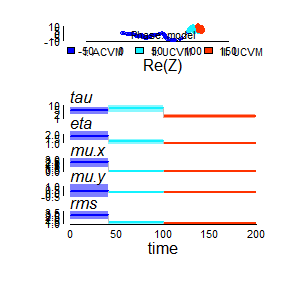
\includegraphics[width=\maxwidth]{figure/SimPhasePlot-1} 

\end{knitrout}

\noindent The estimates are fairly accurate with respect to the true values:
\begin{knitrout}
\definecolor{shadecolor}{rgb}{0.969, 0.969, 0.969}\color{fgcolor}\begin{kframe}
\begin{alltt}
\hlkwd{data.frame}\hlstd{(durations, taus, etas, mus)}
\end{alltt}
\begin{verbatim}
##   durations taus etas mus
## 1        40    3    2   2
## 2        60    3    1   0
## 3       100    1    1   0
\end{verbatim}
\end{kframe}
\end{knitrout}


\section{Kestrel data BCPA}

We perform this analysis now on a portion of the kestrel data analyzed in the Gurarie et al. (in review) manuscript.  The basic steps are the same as above, but the selection occurs across all four models. The portion of data we analyze is:

\begin{knitrout}
\definecolor{shadecolor}{rgb}{0.969, 0.969, 0.969}\color{fgcolor}\begin{kframe}
\begin{alltt}
\hlkwd{data}\hlstd{(Kestrel)}
\hlstd{k} \hlkwb{<-} \hlstd{Kestrel[}\hlnum{3730}\hlopt{:}\hlnum{4150}\hlstd{,]}
\hlkwd{head}\hlstd{(k)}
\end{alltt}
\begin{verbatim}
##        event.id visible           timestamp longitude latitude
## 91352 274467264    true 2012-05-16 01:10:31 -6.556618 37.39312
## 91353 274467265    true 2012-05-16 01:10:32 -6.556670 37.39305
## 91354 274467266    true 2012-05-16 01:10:33 -6.556688 37.39297
## 91355 274467267    true 2012-05-16 01:10:34 -6.556680 37.39283
## 91356 274467268    true 2012-05-16 01:10:35 -6.556643 37.39268
## 91357 274467269    true 2012-05-16 01:10:36 -6.556557 37.39256
##       manually.marked.outlier sensor.type individual.taxon.canonical.name
## 91352                                 gps                  Falco naumanni
## 91353                                 gps                  Falco naumanni
## 91354                                 gps                  Falco naumanni
## 91355                                 gps                  Falco naumanni
## 91356                                 gps                  Falco naumanni
## 91357                                 gps                  Falco naumanni
##       tag.local.identifier     ID          study.name        X       Y
## 91352                  457 B[6.X] Lesser Kestrels EBD 716295.5 4141286
## 91353                  457 B[6.X] Lesser Kestrels EBD 716291.1 4141278
## 91354                  457 B[6.X] Lesser Kestrels EBD 716289.8 4141269
## 91355                  457 B[6.X] Lesser Kestrels EBD 716290.9 4141254
## 91356                  457 B[6.X] Lesser Kestrels EBD 716294.6 4141237
## 91357                  457 B[6.X] Lesser Kestrels EBD 716302.5 4141224
\end{verbatim}
\begin{alltt}
\hlkwd{with}\hlstd{(k,} \hlkwd{scan_track}\hlstd{(}\hlkwc{x}\hlstd{=X,} \hlkwc{y}\hlstd{=Y))}
\end{alltt}
\end{kframe}
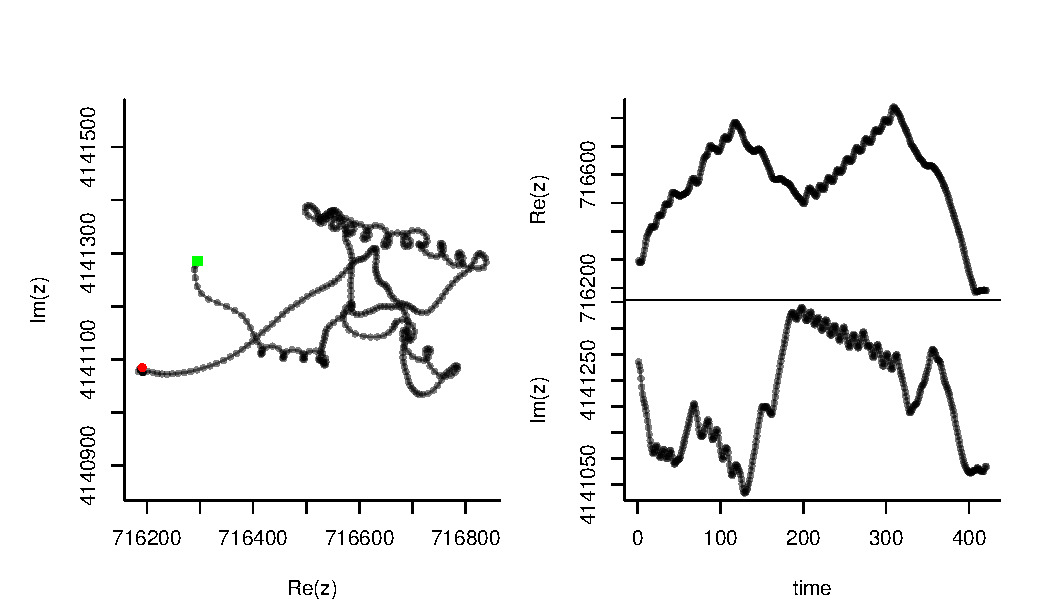
\includegraphics[width=\maxwidth]{figure/subsetKestrel-1} 
\begin{kframe}\begin{alltt}
\hlstd{k}\hlopt{$}\hlstd{T} \hlkwb{<-} \hlkwd{as.numeric}\hlstd{(k}\hlopt{$}\hlstd{timestamp} \hlopt{-} \hlkwd{min}\hlstd{(k}\hlopt{$}\hlstd{timestamp))}
\end{alltt}
\end{kframe}
\end{knitrout}

\noindent The window sweep can take some time. Note that we convert the time to seconds from start (in this case, exactly 420 seconds), which is somewhat more convenient for the analysis (though feeding POSIX objects will also work). 

\begin{knitrout}
\definecolor{shadecolor}{rgb}{0.969, 0.969, 0.969}\color{fgcolor}\begin{kframe}
\begin{alltt}
\hlstd{k.sweep} \hlkwb{<-} \hlkwd{with}\hlstd{(k,} \hlkwd{sweepRACVM}\hlstd{(}\hlkwc{XY}\hlstd{=}\hlkwd{cbind}\hlstd{(X,Y),} \hlkwc{T}\hlstd{=T,} \hlkwc{windowsize} \hlstd{=} \hlnum{50}\hlstd{,} \hlkwc{windowstep} \hlstd{=} \hlnum{5}\hlstd{,}
                              \hlkwc{model} \hlstd{=} \hlstr{"RACVM"}\hlstd{,} \hlkwc{time.units} \hlstd{=} \hlstr{"sec"}\hlstd{,} \hlkwc{progress}\hlstd{=}\hlnum{FALSE}\hlstd{,}
                              \hlkwc{.parallel} \hlstd{=} \hlnum{TRUE}\hlstd{))}
\end{alltt}
\end{kframe}
\end{knitrout}


\noindent Note that the time data are POSIX objects, and it is important to specify the time units of the analysis (in this case, seconds).  We plot the relative likelihoods: 

\begin{knitrout}
\definecolor{shadecolor}{rgb}{0.969, 0.969, 0.969}\color{fgcolor}\begin{kframe}
\begin{alltt}
\hlkwd{plotWindowSweep}\hlstd{(k.sweep)}
\end{alltt}
\end{kframe}
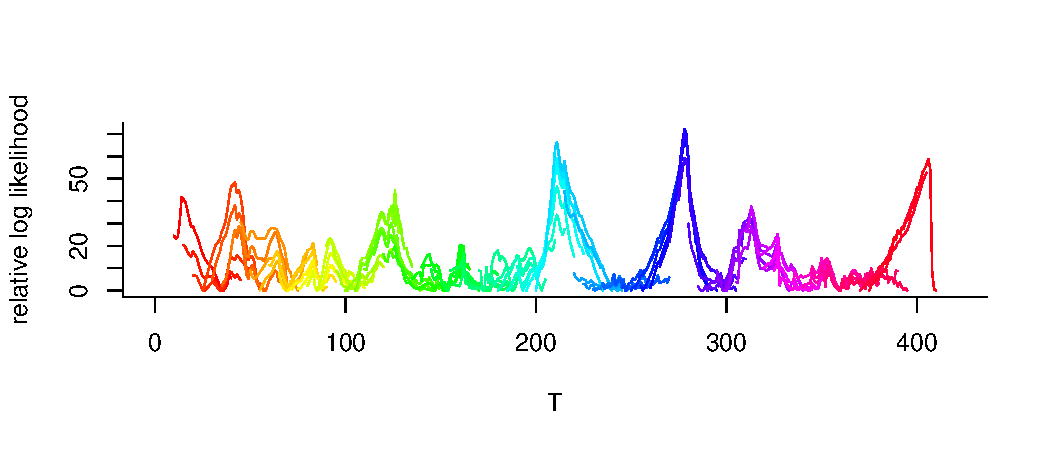
\includegraphics[width=\maxwidth]{figure/plotKestrelSweep-1} 

\end{knitrout}

\noindent There are several clear peaks corresponding to likely change points.  We find candidate change points:

\begin{knitrout}
\definecolor{shadecolor}{rgb}{0.969, 0.969, 0.969}\color{fgcolor}\begin{kframe}
\begin{alltt}
\hlstd{k.CPs} \hlkwb{<-} \hlkwd{findCandidateChangePoints}\hlstd{(}\hlkwc{windowsweep} \hlstd{= k.sweep,} \hlkwc{clusterwidth} \hlstd{=} \hlnum{4}\hlstd{)}
\end{alltt}


{\ttfamily\noindent\itshape\color{messagecolor}{\#\# Note: clustering candidate change points at 4 time units collapsed 38 candidate change points to 26 change points.}}\end{kframe}
\end{knitrout}

\noindent The selected cluster width (4) was the minimum one that did not produce a warning for clusters that were ``too close''.  We now iteratively test all of the change points for parameter values and model changes.  Specifying \texttt{modelset = `all'} is a shortcut for  \texttt{modelset = c(`UCVM', `ACVM', `RCVM', `RACVM')}: 

\begin{knitrout}
\definecolor{shadecolor}{rgb}{0.969, 0.969, 0.969}\color{fgcolor}\begin{kframe}
\begin{alltt}
\hlstd{XY} \hlkwb{<-} \hlkwd{cbind}\hlstd{(k}\hlopt{$}\hlstd{X, k}\hlopt{$}\hlstd{Y)}
\hlstd{k.CPtable} \hlkwb{<-} \hlkwd{getCPtable}\hlstd{(}\hlkwc{CPs} \hlstd{= k.CPs,} \hlkwc{XY} \hlstd{= XY,} \hlkwc{T} \hlstd{= k}\hlopt{$}\hlstd{T,} \hlkwc{modelset} \hlstd{=} \hlstr{"all"}\hlstd{,} \hlkwc{spline}\hlstd{=}\hlnum{TRUE}\hlstd{)}
\end{alltt}


{\ttfamily\noindent\color{warningcolor}{\#\# Warning in min(i1): no non-missing arguments to min; returning Inf}}

{\ttfamily\noindent\color{warningcolor}{\#\# Warning in max(i2): no non-missing arguments to max; returning -Inf}}

{\ttfamily\noindent\bfseries\color{errorcolor}{\#\# Error in min(i1):max(i2): result would be too long a vector}}\end{kframe}
\end{knitrout}
\noindent Note that in this implementation, we chose the option \texttt{spline=TRUE}, as the regularity and apparent precision of these data and the curvature of the track suggest that the spline approximation will give improved estimates of the parameters. 



\begin{knitrout}
\definecolor{shadecolor}{rgb}{0.969, 0.969, 0.969}\color{fgcolor}\begin{kframe}
\begin{alltt}
\hlstd{Z} \hlkwb{<-} \hlstd{XY[,}\hlnum{1}\hlstd{]} \hlopt{+} \hlnum{1i}\hlopt{*}\hlstd{XY[,}\hlnum{2}\hlstd{]}
\hlstd{k.phases} \hlkwb{<-} \hlkwd{getPhases}\hlstd{(k.CPtable,} \hlkwc{T}\hlstd{=k}\hlopt{$}\hlstd{T,} \hlkwc{Z}\hlstd{=Z,} \hlkwc{verbose}\hlstd{=}\hlnum{FALSE}\hlstd{)}
\end{alltt}


{\ttfamily\noindent\bfseries\color{errorcolor}{\#\# Error in getPhases(k.CPtable, T = k\$T, Z = Z, verbose = FALSE): could not find function "{}getPhases"{}}}\begin{alltt}
\hlkwd{summarizePhases}\hlstd{(k.phases)}
\end{alltt}


{\ttfamily\noindent\bfseries\color{errorcolor}{\#\# Error in plyr::llply(phaselist, function(a) \{: object 'k.phases' not found}}\end{kframe}
\end{knitrout}

\begin{knitrout}
\definecolor{shadecolor}{rgb}{0.969, 0.969, 0.969}\color{fgcolor}\begin{kframe}
\begin{alltt}
\hlkwd{layout}\hlstd{(}\hlkwd{c}\hlstd{(}\hlnum{1}\hlstd{,}\hlnum{1}\hlstd{,}\hlnum{1}\hlstd{,}\hlnum{1}\hlstd{,}\hlnum{2}\hlopt{:}\hlnum{6}\hlstd{))}

\hlstd{cols} \hlkwb{<-} \hlkwd{rich.colors}\hlstd{(}\hlkwd{length}\hlstd{(k.phases)}\hlopt{/}\hlnum{2}\hlstd{)}
\end{alltt}


{\ttfamily\noindent\bfseries\color{errorcolor}{\#\# Error in rich.colors(length(k.phases)/2): object 'k.phases' not found}}\begin{alltt}
\hlstd{T.cuts} \hlkwb{<-} \hlkwd{c}\hlstd{(k}\hlopt{$}\hlstd{T[}\hlnum{1}\hlstd{], k.CPtable}\hlopt{$}\hlstd{CP, k}\hlopt{$}\hlstd{T[}\hlkwd{length}\hlstd{(k}\hlopt{$}\hlstd{T)])}
\end{alltt}


{\ttfamily\noindent\bfseries\color{errorcolor}{\#\# Error in eval(expr, envir, enclos): object 'k.CPtable' not found}}\begin{alltt}
\hlstd{Z.cols} \hlkwb{<-} \hlkwd{c}\hlstd{(cols,cols)[}\hlkwd{cut}\hlstd{(k}\hlopt{$}\hlstd{T, T.cuts,} \hlkwc{include.lowest} \hlstd{=} \hlnum{TRUE}\hlstd{)]}
\end{alltt}


{\ttfamily\noindent\bfseries\color{errorcolor}{\#\# Error in eval(expr, envir, enclos): object 'cols' not found}}\begin{alltt}
\hlstd{phaseTable} \hlkwb{<-} \hlkwd{summarizePhases}\hlstd{(k.phases)}
\end{alltt}


{\ttfamily\noindent\bfseries\color{errorcolor}{\#\# Error in plyr::llply(phaselist, function(a) \{: object 'k.phases' not found}}\begin{alltt}
\hlkwd{plot}\hlstd{(Z,} \hlkwc{asp}\hlstd{=}\hlnum{1}\hlstd{,} \hlkwc{type}\hlstd{=}\hlstr{"l"}\hlstd{,} \hlkwc{xpd}\hlstd{=}\hlnum{FALSE}\hlstd{,} \hlkwc{xlab}\hlstd{=}\hlstr{"X (m)"}\hlstd{)}
\hlkwd{points}\hlstd{(Z,} \hlkwc{col}\hlstd{=Z.cols,} \hlkwc{pch}\hlstd{=}\hlnum{21}\hlstd{,} \hlkwc{bg} \hlstd{=} \hlkwd{alpha}\hlstd{(Z.cols,} \hlnum{0.5}\hlstd{),} \hlkwc{cex}\hlstd{=}\hlnum{0.8}\hlstd{)}
\end{alltt}


{\ttfamily\noindent\bfseries\color{errorcolor}{\#\# Error in plot.xy(xy.coords(x, y), type = type, ...): object 'Z.cols' not found}}\begin{alltt}
\hlkwd{legend}\hlstd{(}\hlstr{"topleft"}\hlstd{,} \hlkwc{legend} \hlstd{=} \hlkwd{paste0}\hlstd{(phaseTable}\hlopt{$}\hlstd{phase,} \hlstr{": "}\hlstd{, phaseTable}\hlopt{$}\hlstd{model),}
       \hlkwc{fill}\hlstd{=cols,} \hlkwc{ncol}\hlstd{=}\hlnum{2}\hlstd{,} \hlkwc{bty}\hlstd{=}\hlstr{"n"}\hlstd{,} \hlkwc{title} \hlstd{=} \hlstr{"Phase: model"}\hlstd{)}
\end{alltt}


{\ttfamily\noindent\bfseries\color{errorcolor}{\#\# Error in paste0(phaseTable\$phase, "{}: "{}, phaseTable\$model): object 'phaseTable' not found}}\begin{alltt}
\hlkwd{par}\hlstd{(}\hlkwc{mar}\hlstd{=}\hlkwd{c}\hlstd{(}\hlnum{1}\hlstd{,}\hlnum{0}\hlstd{,}\hlnum{1}\hlstd{,}\hlnum{0}\hlstd{),} \hlkwc{xpd}\hlstd{=}\hlnum{NA}\hlstd{)}
\hlkwd{plotPhaseParameter}\hlstd{(}\hlstr{"tau"}\hlstd{, k.phases,} \hlkwc{ylab}\hlstd{=}\hlstr{"sec"}\hlstd{,} \hlkwc{xaxt}\hlstd{=}\hlstr{"n"}\hlstd{,} \hlkwc{xlab}\hlstd{=}\hlstr{""}\hlstd{,} \hlkwc{col}\hlstd{=cols,} \hlkwc{log}\hlstd{=}\hlstr{"y"}\hlstd{)}
\end{alltt}


{\ttfamily\noindent\bfseries\color{errorcolor}{\#\# Error in inherits(.data, "{}split"{}): object 'k.phases' not found}}\begin{alltt}
\hlkwd{plotPhaseParameter}\hlstd{(}\hlstr{"eta"}\hlstd{, k.phases,}  \hlkwc{ylab}\hlstd{=}\hlstr{"m / sec"}\hlstd{,} \hlkwc{xaxt}\hlstd{=}\hlstr{"n"}\hlstd{,} \hlkwc{xlab}\hlstd{=}\hlstr{""}\hlstd{,}  \hlkwc{col}\hlstd{=cols)}
\end{alltt}


{\ttfamily\noindent\bfseries\color{errorcolor}{\#\# Error in inherits(.data, "{}split"{}): object 'k.phases' not found}}\begin{alltt}
\hlkwd{plotPhaseParameter}\hlstd{(}\hlstr{"omega"}\hlstd{, k.phases,}  \hlkwc{ylab}\hlstd{=}\hlstr{"rad / sec"}\hlstd{,} \hlkwc{xaxt}\hlstd{=}\hlstr{"n"}\hlstd{,} \hlkwc{xlab}\hlstd{=}\hlstr{""}\hlstd{,} \hlkwc{col}\hlstd{=cols)}
\end{alltt}


{\ttfamily\noindent\bfseries\color{errorcolor}{\#\# Error in inherits(.data, "{}split"{}): object 'k.phases' not found}}\begin{alltt}
\hlkwd{plotPhaseParameter}\hlstd{(}\hlstr{"mu.x"}\hlstd{, k.phases,}  \hlkwc{ylab}\hlstd{=}\hlstr{"m / sec"}\hlstd{,} \hlkwc{xaxt}\hlstd{=}\hlstr{"n"}\hlstd{,} \hlkwc{xlab}\hlstd{=}\hlstr{""}\hlstd{,} \hlkwc{col}\hlstd{=cols)}
\end{alltt}


{\ttfamily\noindent\bfseries\color{errorcolor}{\#\# Error in inherits(.data, "{}split"{}): object 'k.phases' not found}}\begin{alltt}
\hlkwd{plotPhaseParameter}\hlstd{(}\hlstr{"mu.y"}\hlstd{, k.phases,}  \hlkwc{ylab}\hlstd{=}\hlstr{"m / sec"}\hlstd{,} \hlkwc{xaxt}\hlstd{=}\hlstr{"n"}\hlstd{,} \hlkwc{xlab}\hlstd{=}\hlstr{""}\hlstd{,} \hlkwc{col}\hlstd{=cols)}
\end{alltt}


{\ttfamily\noindent\bfseries\color{errorcolor}{\#\# Error in inherits(.data, "{}split"{}): object 'k.phases' not found}}\end{kframe}
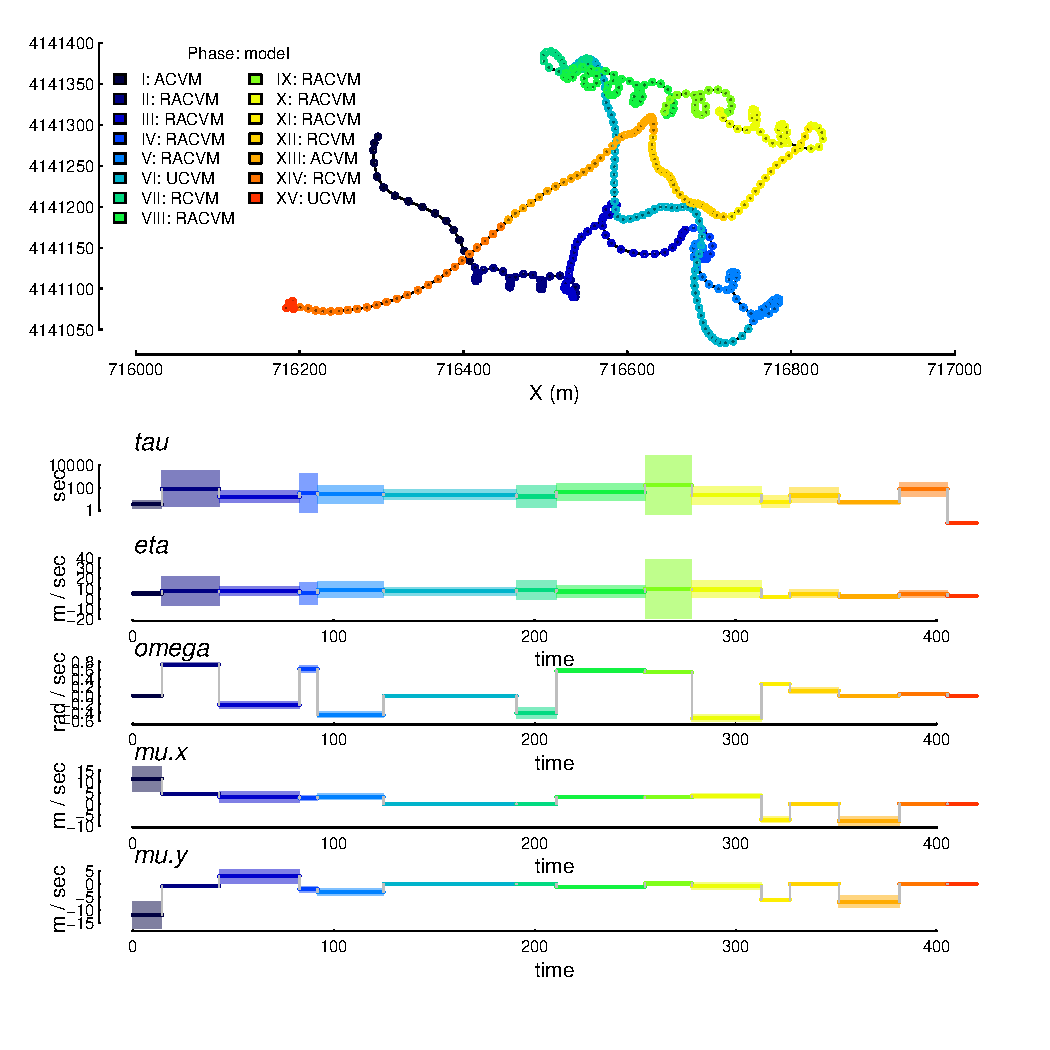
\includegraphics[width=\maxwidth]{figure/kestrelMegaPlot-1} 

\end{knitrout}


\noindent 


\section*{References}

\begin{itemize}

\item[-] Gurarie, E., C.~Fleming, K.~Laidre, W.~Fagan, O.~Ovaskainen (2017) Correlated velocity models as a fundamental unit of animal movement: synthesis and applications \emph{Movement Ecology}. 
\item[-] Johnson, D., J. London, M. -A. Lea, and J. Durban (2008) Continuous-time correlated random walk model for animal telemetry data. Ecology 89(5) 1208-1215.
\item[-] Hern{\'a}ndez-Pliego, J., C.~Rodr{\'i}guez, J.~Bustamante (2015) 'Data from: Why do kestrels soar?', Movebank Data Repository. \url{https://www.datarepository.movebank.org/handle/10255/move.486}
\item[-] Hern{\'a}ndez-Pliego, J., C.~Rodr{\'i}guez, J.~Bustamante (2015) 'Why do kestrels soar?', PLoS ONE 10(12).

\end{itemize}

\section*{Appendix: Properties of the rms estimate}

Issues arise comparing speed parameters directly across model. In any of the advective models, the total speed is contained in the advective component $|\mu|$ and the random component $\eta$, whereas as in the unbiased (or purely rotating) models, the speed is entirely explained by $\eta$.  Thus, to compare across model, the \emph{root mean square} (rms) speed is the best measure, and we are interested in reporting and plotting point estimates and confidence intervals around the rms.  

The formula for the rms is straightforward:  $rms = \sqrt{\eta^2 + \mu_x^2 + \mu_y^2}$.  However, each of those parameters is estimated (and therefore its own random variable) and propagating the error is a little bit tricky. 

If we assume that the estimate of each of the three parameters has a normal distribution with unique means and variances, i.e.~$\widehat{\eta} \sim {\cal N}(\mu_\eta, \sigma_\eta^2)$, etc. Then the variable $\sigma_x^2 X^2 \sim \chi^2_{n.c.}(1, \mu_x^2)$ where $\chi^2_{n.c.}(k, \lambda)$ is the non-central Chi-squared distribution with $k$ degrees of freedom and $\lambda$ non-centrality parameter (and $X$ represents any of the speed estimates). The expectation and variance of this expression are:
\begin{align}
\text{E}(\sigma_x^2 \, X) &= \mu_x^2 + \sigma_x^2\\
\text{var}(\sigma_x^2 \, X) &=  2 \sigma^2  (\sigma^2 + 2 \mu^2)
\end{align}
\noindent Thus, the estimate of the mean square speed (ms), which itself has a non-trivial distribution, has the following mean and variance:
\begin{align}
\text{E}(\widehat{ms}) &= \sum_{i \in \{\mu_x, \mu_y, \eta\}} \mu_i^2 + \sigma_i^2\\
\text{var}(\widehat{ms}) &= \sum_{i \in \{\mu_x, \mu_y, \eta\}} 2 \sigma_i^2  (\sigma_i^2 + 2 \mu_i^2)
\end{align}
\noindent The expectation and variance of the \emph{square root} of $\widehat{ms}$ is well-approximated by the Taylor expansion of the the square root function around the moments:
\begin{align}
\text{E}(\widehat{rms}) &= \sqrt{\text{E}(\widehat{ms})} - {\text{var}(\widehat{ms}) \over 8 (\text{E}(\widehat{ms}))^{3/2}} \\
\text{var}(\widehat{rms}) &= {\text{var}(\widehat{ms}) \over 4 \text{E}(\widehat{ms})}
\end{align}
\noindent Simulations confirm that these are excellent approximations.  


\end{document}
